\documentclass[table, 12pt]{article}
\usepackage[T1]{fontenc}
\usepackage[utf8]{inputenc}
\usepackage[english]{babel}
\usepackage{graphicx}
\usepackage{titlesec}
\usepackage{hyperref}
\usepackage[usenames,dvipsnames]{xcolor}
\usepackage{float}
\usepackage[export]{adjustbox}
\usepackage{longtable}
\usepackage{listings}
\usepackage{alloy}
\usepackage{rotating}

\hyphenation{Te-lan-ga-na}
\hyphenation{an-a-lys-ing}
\hyphenation{a-gron-o-mists}
\hyphenation{a-gron-o-mist}
\titleformat{\paragraph}
{\normalfont\normalsize\bfseries}{\theparagraph}{1em}{}
\titlespacing*{\paragraph}
{0pt}{3.25ex plus 1ex minus .2ex}{1.5ex plus .2ex}


\begin{document}
\begin{titlepage}
    \centering
    {\scshape\large AY 2021/2022 \par}
    \vfill
    
\includegraphics[width=100pt]{assets/logo-polimi-new}\par\vspace{1cm}
    {\scshape\LARGE Politecnico di Milano \par}
    \vspace{1.5cm}
    {\huge\bfseries RASD\@: Requirement Analysis
        and Specification Document \par}
    \vspace{2cm}
    {\Large {Ottavia Belotti\quad Alessio Braccini\quad Riccardo Izzo}\par}
    \vfill
    {\large Professor\par
        Elisabetta \textsc{Di Nitto}}
    \vfill
    {\large \textbf{Version 1.1}\\ \today \par}
\end{titlepage}

\hypersetup{%
    pdfborder = {0 0 0}
}

\thispagestyle{plain}
\pagenumbering{gobble}
\mbox{}
\newpage
\pagenumbering{roman}
\tableofcontents
\newpage
\pagenumbering{arabic}

\section{Introduction}
\emph{Data-dRiven PrEdictive FArMing}, also known as \emph{DREAM}, is a project presented by UNDP India and Healthsites initiative, promoted by Telangana's government.
The aim of the project is to enhance the farm system and the entire food supply chain with an IT supporting application. 
This arises from modern challenges like climate change and the foreseen population growth that have underlined the critical issues of the modern system making necessary a complete revision.


\subsection{Purpose} %goals of the project
\emph{DREAM} aims to support the work categories involved into the farming industry by providing them relevant and up-to-date data about farms activity's performance. 
The main stakeholders are: Telangana policy makers, farmers and agronomists.
The goal is to develop a data-driven application with the help of IT partners.
Telangana's state already collect important data concerning wheather forecast; these data are publicly available with a live rainfall map on the official government website.
Other data can be collected through humidity sensors deployed all over the territory and through the water irrigation system.

Agriculture has a main role in India's economy, more than half of the population depends on it and about a fifth is below the poverty line.
Furthermore, as a significant increment in population is expected by 2050 (\emph{UN}'s esteem), food demand is going to significantly increase.
Telangana needs an efficient application to increase the general productivity of the farm system.

The user base is expected to include a large part of Telangana's population, bringing together people with different knowledge backgrounds, such as people directly working in the agricolture field up to political figures.

\subsubsection{Goals}
\newcounter{goalCtr}
\underline{Shared goals}
\begin{enumerate}
    \item  \textbf{(\stepcounter{goalCtr}G\arabic{goalCtr}) Reach out to farmers in need of help} \\ Farmers that struggle with their cultivation wish to be helped and turn around their business in a positive way, since their income depend on that. At the same time, given the forseen food supply demand, policy makers and agronomists strive for reaching the maximum potential of every suppliers.
\end{enumerate}
\underline{Telangana's policy makers}
\begin{enumerate}
    \item \textbf{(\stepcounter{goalCtr}G\arabic{goalCtr}) Identification of well-performing  and under-performing farmers}\\
    Main goal of the policy makers is to identify farmers that are resilient to meteorological adverse events.
    %This can be done comparing the productivity ratio defined as the produced amount per product in adverse condition over the amount in standard conditions.
    These farmers will receive special incentives as a compensation for being asked to share their own best practices with the policy maker and agronomist that might apply them on a larger scale later.

    Identify farmers that are performing badly in order to seek the help for them to get back on track. In fact, they are the ones that need to be helped by the agronomists and by regulation promoted by policy makers promoting better practices.
    \item \textbf{(\stepcounter{goalCtr}G\arabic{goalCtr}) Visualize the results of steering initiatives}\\
    Visualize and evaluate the results produced by the steering initiatives from agronomists and good farmers in order to assess which are resulting useful and actually improving the food production system, so that those practices can be applied on a larger scale.
\end{enumerate}
\underline{Farmers}
\begin{enumerate}
    \item \textbf{(\stepcounter{goalCtr}G\arabic{goalCtr}) Visualize relevant data for the business}\\
    Visualize important data like weather forecast and personalized suggestion about specific crops or fertilizers.
    All data are based on location and type of production.
    \item \textbf{(\stepcounter{goalCtr}G\arabic{goalCtr}) Keep track of the production}\\
    Insert data about their production to identify trends of their own doings, especially bad ones undermining their revenue. Register every type of problem they're experiencing for further inspection with the help of experts in the field.
    \item \textbf{(\stepcounter{goalCtr}G\arabic{goalCtr}) Request for help/suggestion}\\
    Farmers can request help with a text message that will be sent directly to the agronomists responsible of the area to better their practice both in critical conditions and for improvement purposes. %Thanks to this, the farmers are not required to know directly the contact of one of the agronomists, because the system will provide the contacts of the area they need automatically.
    \item \textbf{(\stepcounter{goalCtr}G\arabic{goalCtr}) Create and participate in discussions concerning the agricolture field}\\
    Create forums to discuss with the other farmers. This feature shall allow a farmer-user to choose the name of a new topic they wish to introduce in the forum and to join all already open discussions. The purpose of this is to ease the cultivation-related knowledge spreading from which every farmer would benefit.
\end{enumerate}

\underline{Agronomists}
\begin{enumerate}
    \item \textbf{(\stepcounter{goalCtr}G\arabic{goalCtr}) Receive requests for help/suggestion all in one place}\\
    Here the agronomist can manage all the incoming request for help or suggestion and will have an higher chance of intervening promptly in critical situations before it's too late. In fact, having just one place in which all the requests that need attention are cumulated makes easier for them to not miss any, rather than losing them because of the different means they could come from and in a unstructured way.
    \item \textbf{(\stepcounter{goalCtr}G\arabic{goalCtr}) Visualize area statistics}\\
    Keep track of the area general performance through a list of best-performing farmers and visualize data about whether forecast.
    %The list of best-performing farmers is based on the productivity over a selected period of time.
    \item \textbf{(\stepcounter{goalCtr}G\arabic{goalCtr}) Easy daily planning procedure}\\
    The daily plan consists in a list of farms to be visited during the day.
    Since, by regulations, every farm must be visited at least twice a year, with particular attention to the under-performing ones that should be visited more often, agronomists wish to be suggested of which are the farms that are due to be visited or the ones that have not been visited yet during the year.
\end{enumerate}

\subsection{Scope} %analysis of the world and shared phenomena
%ADD: basic service and advanced functionalities
\subsubsection*{Phenomena controlled by the Machine}
\newcounter{machineP}
\rowcolors{2}{PineGreen!25}{}
\begin{center}
\begin{tabular}{|c|p{0.70\textwidth}|c|}
    \hline
    \textbf{ID} & \textbf{Phenomenom} & \textbf{Shared} \\\hline\hline
    \stepcounter{machineP}
    M\arabic{machineP} & Visualize data concerning weather, land, performance & Yes\\\hline
    \stepcounter{machineP}
    M\arabic{machineP} & User is given statistic data & Yes \\\hline %might remove this
    \stepcounter{machineP}
    M\arabic{machineP} & User is notified of unread requests for help or suggestions & Yes \\\hline
    \stepcounter{machineP}
    M\arabic{machineP} & User is suggested about which farms need to be visited & Yes \\\hline
    \stepcounter{machineP}
    M\arabic{machineP} & User is presented with news that might be relevant to their business & Yes \\\hline
    \hline
\end{tabular}
\end{center}

\subsubsection*{Phenomena controlled by the World}
\newcounter{worldP}
\begin{center}
    \rowcolors{2}{PineGreen!25}{}
    \begin{tabular}{|c|p{0.70\textwidth}|c|}
        \hline
        \textbf{ID} & \textbf{Phenomenom} & \textbf{Shared} \\\hline\hline
        \stepcounter{worldP}
        W\arabic{worldP} & User logs in & Yes\\\hline
        \stepcounter{worldP}
        W\arabic{worldP} & User queries for the farmers ranking & Yes \\\hline
        \stepcounter{worldP}
        W\arabic{worldP} & User queries for statistic data from humidity sensors & Yes \\\hline
        \stepcounter{worldP}
        W\arabic{worldP} & User queries for statistic data from wather irrigation sensors & Yes \\\hline
        \stepcounter{worldP}
        W\arabic{worldP} & User sends a request for help to an agronomist & Yes\\\hline
        \stepcounter{worldP}
        W\arabic{worldP} & User creates topic in forum & Yes\\\hline 
        \stepcounter{worldP}
        W\arabic{worldP} & User joins a discussion in forum & Yes \\\hline
        \stepcounter{worldP}
        W\arabic{worldP} & User inserts post on the forum & Yes\\\hline
        \stepcounter{worldP}
        W\arabic{worldP} & User updates daily plan & Yes\\\hline      
        \stepcounter{worldP}
        W\arabic{worldP} & User confirms daily plan & Yes \\\hline
        \stepcounter{worldP}
        W\arabic{worldP} & User pays a visit to a farm & No \\\hline
        \stepcounter{worldP}
        W\arabic{worldP} & User receives a visit in his/her own farm & No \\\hline
        \stepcounter{worldP}
        W\arabic{worldP} & User reads help requests & Yes \\\hline
        \stepcounter{worldP}
        W\arabic{worldP} & User replies to request for help & Yes \\\hline   
        \stepcounter{worldP}
        W\arabic{worldP} & User checks weather forecast & Yes\\\hline
        \stepcounter{worldP}
        W\arabic{worldP} & User checks news about crop & Yes \\\hline
        \hline
    \end{tabular}
\end{center}

\subsection{Definitions, acronyms, abbreviations}
\subsubsection*{Definitions}
\begin{itemize}
    \item \textbf{Agronomist}: scientist in the agricoluture field. Their main professional role is to make sure of the well-being of crops and recommend solutions to farmers in need of help with their cultivations 
    \item \textbf{Daily plan}: a schedule of the activities to be done during the day, each of them planned out with their own starting time and location
    \item \textbf{Farmer}: workers that own or manage a farm with the intention of selling at least a part of their own production
    \item \textbf{Forum}: online spot enabling users to meet and exchange ideas, share tips, express concerns and arise issues related to topics that comply to the purpose of the forum itself
    \item \textbf{Policy Maker}: political figure responsible or involved in formulating policies, specifically food chain supply policies in this document
    \item \textbf{Production}: in this particular document, it's any type of edible result coming from crop
    \item \textbf{Telangana}: Indian state promoting the \emph{DREAM} project
    \item \textbf{User}: either Policy Makers, Farmers or Agronomists that will use the app  
\end{itemize}
\subsubsection*{Acronyms}
\begin{itemize}
    \item \textbf{AES}: Advanced Encryption Standard
    \item \textbf{API}: Application Programming Interface
    \item \textbf{CE}: Conformité Européenne
    \item \textbf{DBMS}: Database Management System
    \item \textbf{DREAM}: \emph{Data-driven predictive farming} project
    \item \textbf{GPS}: Global Positioning System
    \item \textbf{IT}: Information Technology
    \item \textbf{MTTF}: Mean Time To Failure
    \item \textbf{MTTR}: Mean Time To Repair
    \item \textbf{PDPA}: Personal Data Protection Act 
    \item \textbf{RASD}: Requirement Analysis and Specification Document
    \item \textbf{SSL}: Secure Sockets Layer
    \item \textbf{UML}: Unified Modeling Language
\end{itemize}
\subsection{Revision history}
\subsection{Reference documents}
\begin{itemize}
    \item Specification document: "Assignment RDD AY 2021-2022"
    \item Alloy documentation: https://alloytools.org/documentation.html
    \item UML documentation: https://www.uml-diagrams.org/
    \item BPMN documentation: https://www.bpmn.org/
    \item Paper: "The World and the Machine" by M. Jackson and P. Zave   
\end{itemize}

\subsection{Document structure}
\begin{itemize}
    \item \textbf{Section 1} gives an introduction about the problem to tackle and about which functionalities will be implemented in the final product in order to comply to the users' needs.
    \item \textbf{Section 2} contains the overall description of the whole project, presenting it in a more formal way through class diagrams which will show the main flows and extepcted interactions between the user and the system. Furthermore, there will be presented: the so-called \emph{actors} divided into the different types of user that will populate the application; the expected functionalities and the domain assumptions taken in consideration throughout the whole project, from the specification phase to the actual developing phase. To exemplify all the above, typical scenarios will be provided.
    \item \textbf{Section 3} delves deeply into the topics presented in \emph{Section 2}, in order to be more clear in setting the bounds between what the application must implement and what not. It will show functional and non-functional requirements. The former will be presented through some use-cases as meaningful examples; while the latter will be disclosed by analysing performance, design choices and software system features that the project shall have.
    \item \textbf{Section 4} presents the Alloy code briefly explainig the purpose of it in modeling the given problem.
\end{itemize}
\newpage
\section{Overall Description}
\subsection{Product perspective}
DREAM is a system that offers the functionalities described in the \textit{Product Functions (\ref{product_functions})} section.
It manages to use some external interfaces, for more details refers to the \textit{Software Interfaces (\ref{software_interfaces})} section.
In the following subsections we can see a list of the most common scenarios \textit{(\ref{scenarios})} and an high-level class diagram \textit{(\ref{class_diagram})} that shows the basic structure of the system.
\subsubsection{Scenarios}
\label{scenarios}
\begin{enumerate}

    \item Aanya has just passed her test to become a policy maker and wants to consult the app.
    To do so she decides to download and install DREAM in order to visualize the data concerning her job.
    \begin{itemize}
        \item She opens the app and click on the "Sign Up" button
        \item She inserts all her data in order to fill every mandatory field and presses the "Confirm" button
        \item The system verifies that the e-mail isn't already present in the database. Since there isn't an entry for her e-mail yet, it allows the registration and shows a confirmation message to Aanya's mailbox
        \item She checks her mailbox in order to verify that the procedure ended successfully
    \end{itemize}

    \item Apu is an expert policy maker, he wants to know what are the latest data regarding soil humidity and water irrigation.
    \begin{itemize}
        \item He takes his phone and logs in DREAM app 
        \item He presses the "Visualize Data" button
        \item The system retrieves data from a database and shows him the soil moisture and the consumed liters of water by the irrigation system thorughtout graphs that computes the average quantities across the Country in a span of one year
        \item He wishes to have more detailed information about the soil humidity and the water irrigation in Adilabad district since he read an alarming report about that region.
        He choses it from the menu and sets the time span at two weeks
        \item The system gives him new graphs reporting only data about soil humidity and water used for irrigation retrieved by Adilabad's sensors in the last two weeks
        \item He analyzes them and decides that he will talk about it later with a colleague, then he returns to the home page
    \end{itemize} 

    \item Pajeet is one of the main policy makers in the state of Telangana.
    He wants to distribute special incentives to the best farmers and to do this he decides
    to open the app and visualize the data.
    \begin{itemize}
        \item He opens the app on his device. Since he's already registered, he logs in
        \item The system shows the homepage for a policy maker user
        \item He visualizes the ranking of the well-performing farmers
        \item He clicks on the name of a farmer
        \item Now the system shows the profile of the selected farmer
        \item Here the policy maker can find useful contact information such as phone number (if it has been given by the farmer) and email
        \item He takes note of the desirable contact information and closes the app
    \end{itemize}

    \item Chandran is an old farmer that has been cultivating mais for all his life. He has recently decided to move out from his previous field in order to give it to his son, Aakesh. Aakesh has already his own land near his dad's one, so he wants to add the new gifted area to his DREAM account. Furthermore, he found out that wheat is more productive and more bug-resistant than mais, so he also wants to change the crop type for both the lands from mais to wheat.
    \begin{itemize}
        \item He logs in DREAM app
        \item He presses the "Profile Edit" button in order to change his area and crop type
        \item He changes the two value by inserting a new area and a new crop type
        \item He confirms by pressing the "Confirm" button
    \end{itemize}

    \item Sahil is a farmer that would like to share some best-practices about a particular product that he has cultivated during the last year.
    He decides to open a new discussion on the forum.
    \begin{itemize}
        \item He opens the app on his device. Since he's already registered, he logs in
        \item The system shows the homepage for a farmer user
        \item He clicks on the "Forum" button and access the forum section
        \item Now he clicks on the "Create new topic" button where he can select the name of the discussion
        \item He posts a new message in the discussion
        \item Finally some time later he checks if someone has joined his topic and replied to him
    \end{itemize}

    \item Damayanti is a farmer that would like to improve the productivity of his farm.
    To do so he decides to consult the section regarding the suggestions on specific crops to plant or specific fertilizers to use.
    \begin{itemize}
        \item He opens the app on his device, if he is already registered he logs in
        \item The system shows the homepage for a farmer user
        \item He clicks on the "News" button and access the news section
        \item Here he visualizes suggestions based on his type of production and on his location
        \item If he is not satisfied, then he clicks on the "Request for help" button to send a message
        \item Here the app suggests him the agronomist responsible of the area and opens a text section where he can type his requests for suggestions
        \item Otherwise, he takes note from the article he read
        \item He closes the app
    \end{itemize}

    \item Chakrika is a young farmer and decided to insert the data regarding last week production.
    \begin{itemize}
        \item She takes her computer and logs in DREAM
        \item The system shows her the farmers home page
        \item She presses the "Insert production data" button
        \item She inserts the total quantity of rice harvested last week 
        \item She checks the inserted data and finally press the "Confirm" button 
        \item The system sends her back to the home page
    \end{itemize}

    \item Shaleena is an agronomist responsible of Mahbubnagar, one of the biggest region in Telangana.
    She wants to compose the daily plan to decides which farms to visit today and for this reason she decides to open the app.
    \begin{itemize}
        \item She opens the app on his device, if she is already registered she logs in
        \item The system shows the homepage for an agronomist user
        \item She clicks on the "Daily plan" button and access the new section
        \item She adds the farms she wants to visit to the daily plan by choosing them from the list of available ones
        \item Now the system shows the addresses and the date of the last visit of the selected farms
        \item She takes note of the addresses and close the app
    \end{itemize}
    \item Chaitanya is an agronomist that after a hard day of work wants to update the daily plan on the app.
    At the end of the day she realizes that she has visited three farms instead of the two indicated in the daily plan.
    \begin{itemize}
        \item She opens the app on his device, if she is already registered she logs in
        \item The system shows the homepage for an agronomist user
        \item She clicks on the "Daily plan" button and access the new section
        \item Here she can visualize the daily plan
        \item She can click on the "Add" or on the "Remove" button
        \item In case of "Add" the system would redirect her to the list of available ones, in case of "Remove" she can delete a farm 
        from the list simply by clicking on the cross at the right
        \item She clicks on the "Confirm" button to validate the daily plan
        \item The system returns to the homepage
        \item Finally she closes the app
    \end{itemize}
    
    \item Pradeep is an agronomist who wants to take care about help requests before going to work.
    \begin{itemize}
        \item He opens the app on his device, if he is already registered he logs in
        \item The system shows the homepage for an agronomist user
        \item He clicks on the "Mail box" button and access the new section
        \item Here he visualizes a list of help requests
        \item By clicking on a help request he can visualize the request and answer it
        \item He does this for every help request until they are finished
        \item Finally he closes the app and begins his working day
    \end{itemize} 

    \item Sonya is an agronomist that want to check who are the best farmers of her responsibility area.
    \begin{itemize}
        \item She take her IT device and log in the system 
        \item She can already see who are the top farmers of the area
        \item She press the widget and look deeply the ranking
        \item She press the "Home" button to return to home page
    \end{itemize}
\end{enumerate}


\subsubsection{Class diagram}
\label{class_diagram}
A UML class diagram describes the main entities in the system.
Three types of actors can access the system: farmers, policy makers and agronomists.
During the sign-up, they all create a user account with basic information such as username, password and e-mail.
At this point, users are requested to choose what type of account to create. It is crucial that phisycal users register themselves accordingly to their job to ensure that the system works properly. Furthermore, this choice affects the next steps in the registration phase; for example, to complete the registration, farmers need to specify the position of their farm and what type of crop they grow, whereas agronomists must declare their area of responsibility.

The system provides several functionalities tailored for the type of user, one of these is the forum for the farmers. When the farmers select the forum section, they are presented with the topics that are already active. For each topic, the discussion that has evolved through time can be seen: it's composed by the original post and its replies from other users. From here, the user can join an already ongoing discussion or create a new one generating a new topic and post the first message for it.

Another functionality is the \textit{daily plan} feature for the agronomists.
A daily plan is a list of farms that an agronomist has decided to visit on a particular day of the year, it has a date and a status flag that indicates whether the plan has already been confirmed or not\footnotemark. %The schedule can be planned from the day before the actual visit and be confirmed until 23:59 of the visiting day. If the agronomist fills the plan and doesn't confirm it before the time limit expires, then the system will automatically assumes that the schedule has been followed and will archive it at the end of the day. 
For the planner, agronomists have access to the list of farmers currently in their area of responsibility and registered to the app.
\footnotetext{More technical details can be found in the DD document.}

Finally, there are various types of data that can be visualized and analyzed by the users
depending on the type of their account.
There are four types of data:
\begin{itemize}
    \item \textbf{Soil humidity sensors data}\\
    Acquired by the sensors distributed all over the territory, they report values that represent the soil moisture level of the land they cover.
    \item \textbf{Weather forecast data}\\
    Meteorological short-term and long-term forecast acquired by Telangana's government and displayed on their official website. They are comprehensive of temperature, rainfall probability and quantity, direction and strength of the wind and air humidity.
    \item \textbf{Water irrigation data}\\
    Acquired by the water irrigation system installed in the farms, the only significant value is the amount of water used by the system during the day.
    \item \textbf{Production data}\\
    Provided by the farmers, this type of data is displayed as a table that maps the type of cultivated product to the sown amount and the respective harvested quantity.
    \item \textbf{Report}\\
    Reports are written by Agronomists whenever they lead new initiatives aiming to better the results of cultivation in their area. The reports include a detailed explanation of the content of the initiative and the feedback they've been collecting since their attuation.
\end{itemize}
\begin{center}
    \begin{figure}[H]
        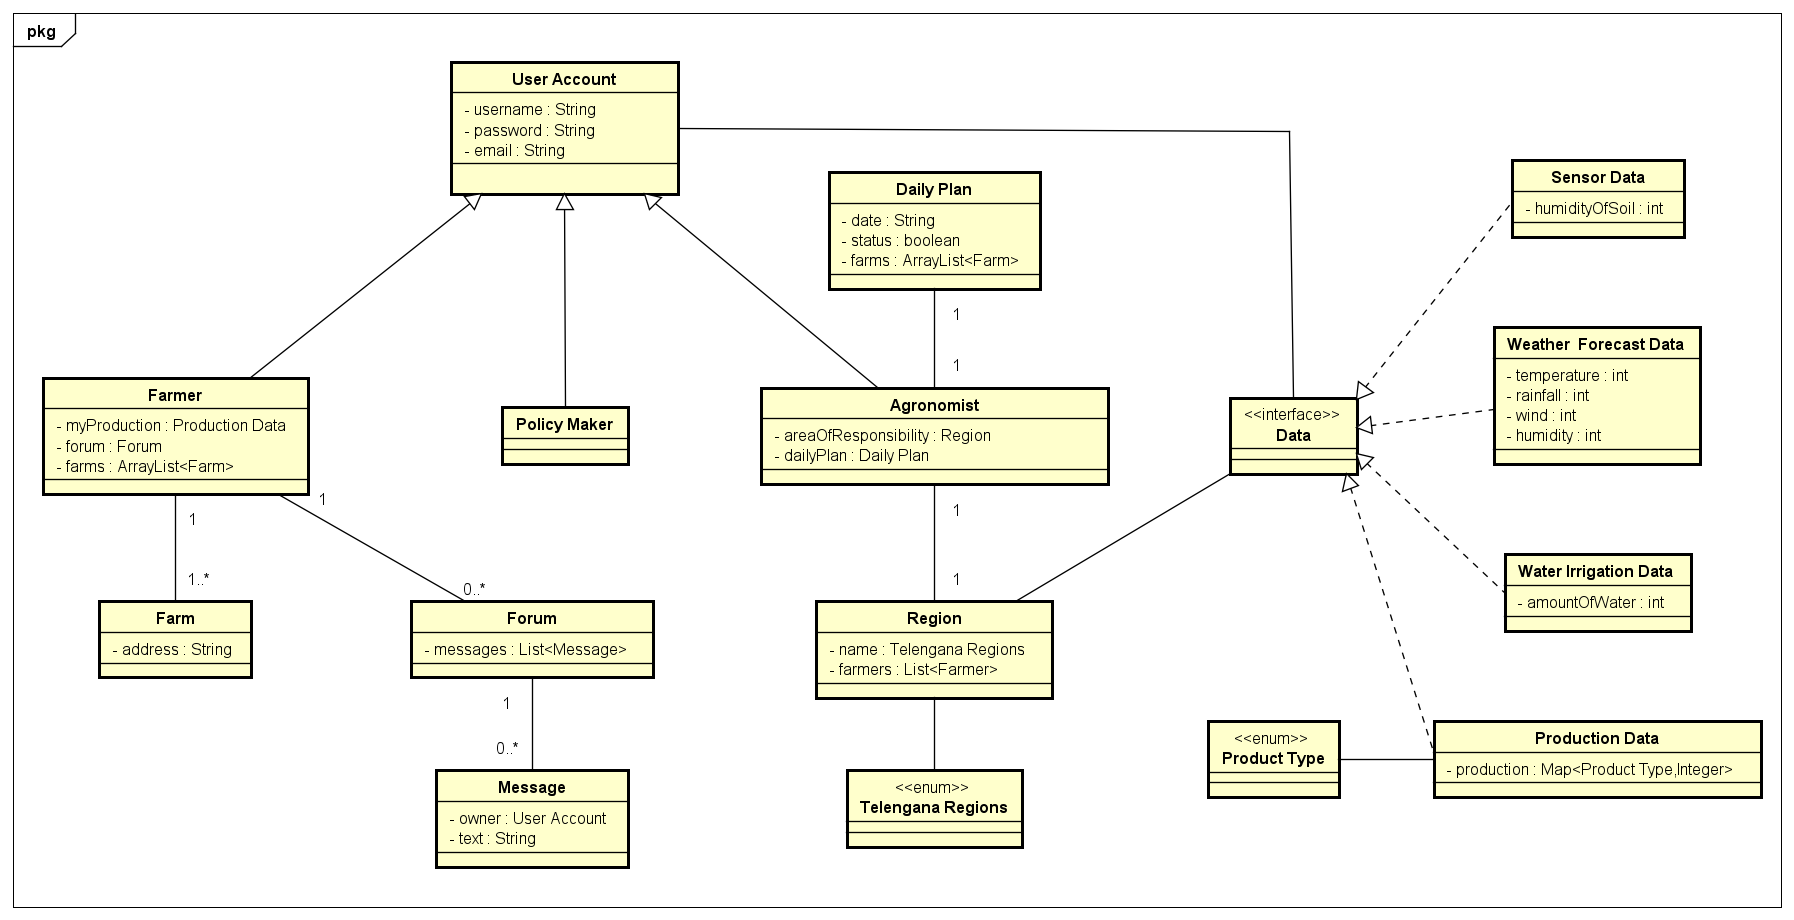
\includegraphics[scale=0.45, center]{assets/UML/UML.png}
        \caption{High-level UML}
        \label{fig: UML}
    \end{figure}
\end{center}
\subsection{Product functions}
\label{product_functions}
\subsubsection{Sign-up and shared functions}
\begin{itemize}
    \item \textbf{Sign-up:} let the user sign-up thorugh an email and a password, creating a profile tailored for the user's job. Specify the area in which they live and what type of cultivation they manage\footnotemark. The adding of a farmland is done by inserting its coordinates (raw coordinates or by selecting a spot on the map) into the app, since it's difficult to find a location through an address in rural areas.
    \footnotetext{The positioning of a farm is tackled more in depth in the DD document.}
    \begin{center}
        \begin{figure}[!h]
            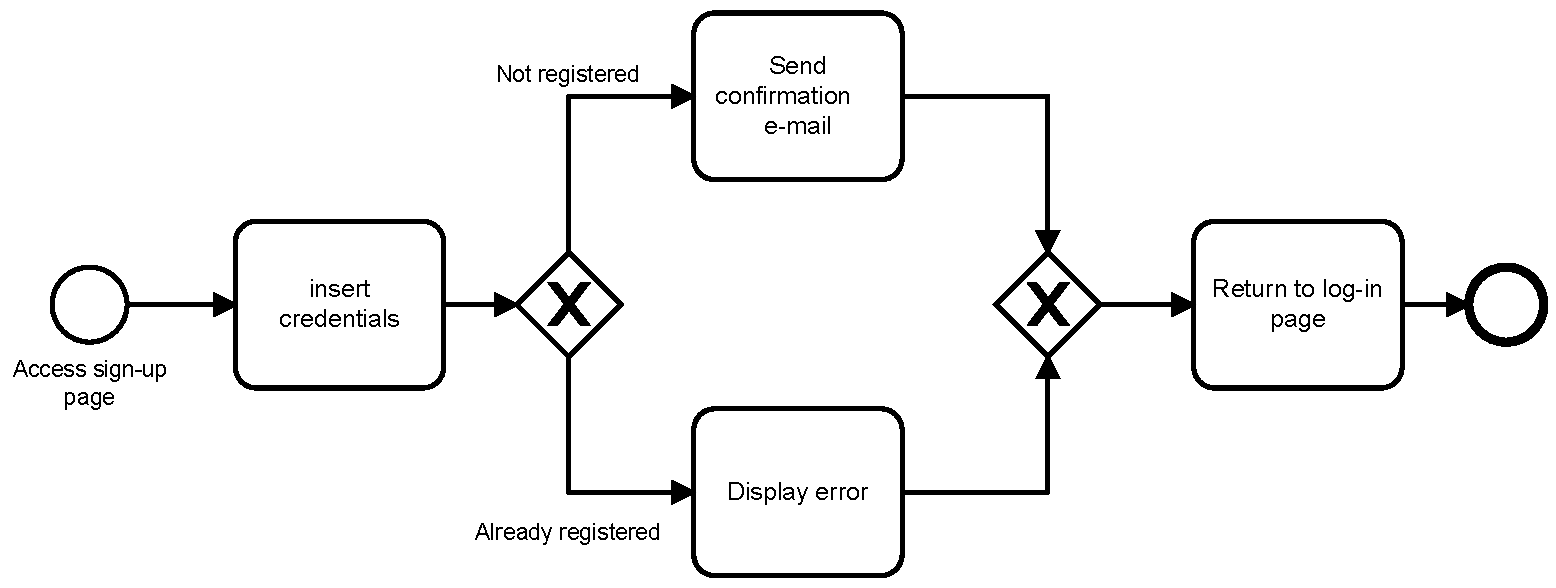
\includegraphics[width=\textwidth]{assets/BPMN/SignUpBpmn}
            \caption{Sign Up BPMN}
            \label{fig: singup}
        \end{figure}
    \end{center}
\end{itemize}
\subsubsection{Policy makers functions}
\begin{itemize}                                 
    \item \textbf{Visualize relevant data and initiatives:} let the policy makers know a variety of data like the performances of the farmers by grouping them in a rank to know who are the farmers that are performing well and who are the worst one mainly based upon the production data provided by them.
    Policy makers can also visualize the steering iniziatives presented by the agronomists' reports that are collected into a specific subsection of their application.
\end{itemize}
\subsubsection{Farmers functions}
\begin{itemize}
    \item \textbf{Getting information about the agricolture field:} allow farmers to visualize news relevant to their business interests such as: wheather forecast for the day or for the next few days, articles posted on major online farming magazines that are related to their own crop type and specific fertilizers for their needs.
    \item \textbf{Agronomists Interactions:} allow farmers to send messages to the agronomist.
    \item \textbf{Building a useful community on the forum:} allow farmers to create a new topic or reply to a message in the dedicated forum.
\end{itemize}
\begin{center}
    \begin{figure}[H]
        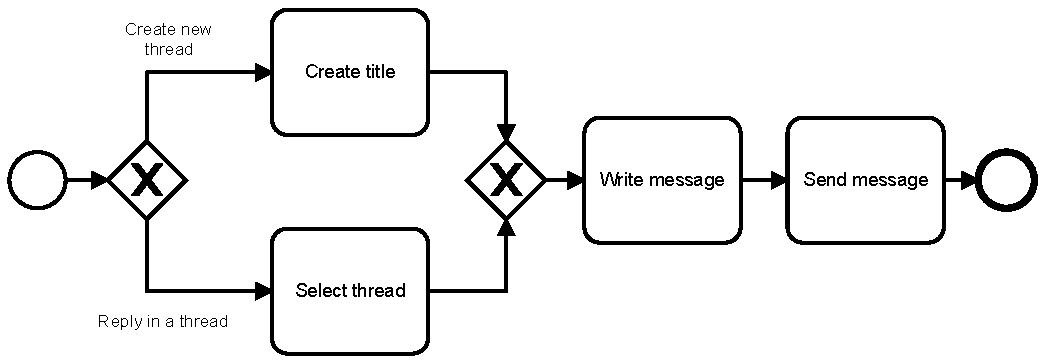
\includegraphics[width=\textwidth]{assets/BPMN/ForumBpmn}
        \caption{Forum BPMN}
        \label{fig: forum}
    \end{figure}
\end{center}
\subsubsection{Agronomists functions}
\begin{itemize}
    \item \textbf{Area functions:} allow the agronomists to insert their responsibility area and visualize related data like wheather forecast or the rank of the farmers in that region.
    \item \textbf{Manage farmers requests:} agronomists reply to farmers' requests for help or suggestion.
    \item \textbf{Manage daily plan:} allow the agronomist to make their daily plan by registring the scheduled visits to the farmers. At the end of the day an agronomist must confirm if they were able to complete the plan or specify the deviations occurred during the day. Updating the daily plan because of a deviation means either adding a farm that has been visited during that day that was not originally in the plan, or removing one from the schedule if the agronomist has not been able to pay a visit that same day.  
\end{itemize}
\begin{center}
    \begin{figure}[H]
        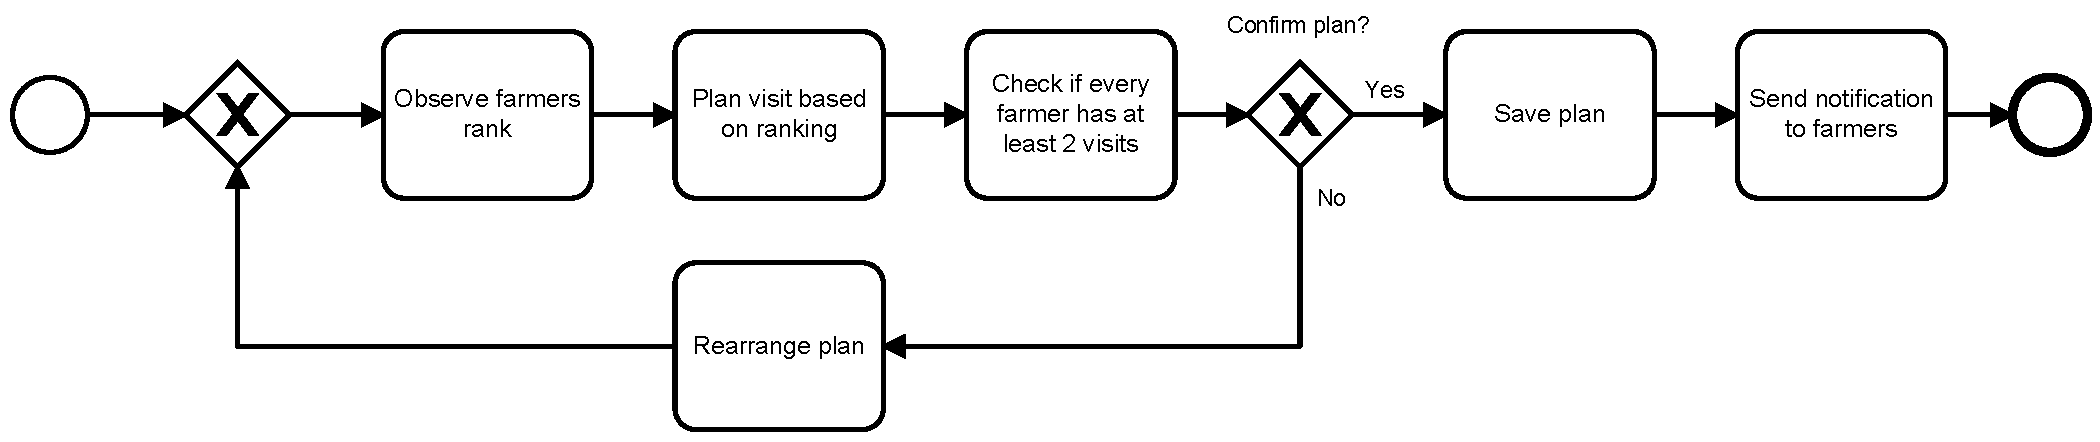
\includegraphics[width=\textwidth]{assets/BPMN/DailyPlanBpmn}
        \caption{Daily plan BPMN}
        \label{fig: dailyplan}
    \end{figure}
\end{center}

\subsection{User characteristics}
The application has been thought for the three different user categories that follows:
\begin{itemize}
    \item \textbf{Policy makers} are government's employees that are in charge of analysing the general agricolture trends among all the districts in Telangana, then promote based state-wide policies to better the whole food system. Their main goal is not only to secure the current provision, but also to identify now the best practices that will lead to a flourishing food production in the future. By doing so, the plan is to grow more resilient and profitable crops and prepare the lands to face future menaces, for instance the climate that is getting more hostile or the foreseen increment of the food demand. As a consequence, they want to be notified about the best performing farmers in order to contact them and get more insight from them about their procedures, with the aim to acquire best practises to be shared and applied on a larger scale. At the same time, they need to know who, on the other hand, is performing particularly badly, so that they can be given the help they need to better their results, since obtaining the foresaid goal requires the structure to run smoothly in all its parts. 
    Policy makers also need a feedback system that let them be aware of the true impact \textit{a posteriori} of the initiatives carried out by the agronomists in collaboration with the knowledge and practice of the best farmers.
    \item \textbf{Farmers} are interested in functionalities that will help with their day-to-day life at work, so they would like to receive in one place all the information about the weather to plan before hand the work day and useful data, like suggestions and news about the specific crop they cultivate, if some crop's illness is spreading in their area and how to treat it, which fertilizers boost the plant's production, etc. Moreover, they should insert data about their own production and ask for help to a regional agronomist through the app if it's needed. Being part of a larger community of people that share the same purpose (such as being more productive) brings more knowledge in general, so it's easier for the farmers to get in touch with their collegues that grow the same crops and might have faced the same challenges they do through the in-app forum. The feature allows them to enlarge their pool of acquaintances and brings them together online, even though they might be kilometers away from each other.
    \item \textbf{Agronomists} are the experts in the agricolture field, so the main function needed for them is the possibility of helping out the farmers that reach out to them. Each agronomist is in charge of a specific geographical area in Telangana, in order to be efficiently present on the territory in a fair and useful way according to the actual helping demand. In fact, they visit each farm spread among their area at least twice a year. That said, agronomists would like some functionalities that help them planning out their trips on the field in an simple yet flexible way. Furthermore, they would like to be notified of the farms' performace, especially the ones scoring poor results in order to plan their visits more often for those, depending on the problem their facing. Nonetheless, in order to make a complete and exhaustive report about the area productivity for the central government, they are also interested into acknowledging the top performing farms. %wheather forecast? go deeper in explaining daily plan funct?
\end{itemize}
\subsection{Assumptions, dependencies and constraints}
\newcounter{assumptionCtr}
\begin{itemize}
    \item \stepcounter{assumptionCtr}D\arabic{assumptionCtr}: Agronomists actually stick to the scheduled daily plan
    \item \stepcounter{assumptionCtr}D\arabic{assumptionCtr}: Agronomists correct their schedule at the end of the day if deviations occur
    \item \stepcounter{assumptionCtr}D\arabic{assumptionCtr}: Each user registers only once, according to their job, and always feeds correct information to the app
    \item \stepcounter{assumptionCtr}D\arabic{assumptionCtr}: The internet connection works properly when the application is being used\footnotemark
    \item \stepcounter{assumptionCtr}D\arabic{assumptionCtr}: The sensors measuring humidity level of the soil work properly, with at most an error of 1\%
    \item \stepcounter{assumptionCtr}D\arabic{assumptionCtr}: Weather forecasts are accurate up to a 80\% for the short-term and up to 60\% on the long-term
    \item \stepcounter{assumptionCtr}D\arabic{assumptionCtr}: Water irrigation system send the information accurately, with an error of at most 1\%
    \item \stepcounter{assumptionCtr}D\arabic{assumptionCtr}: Agronomists always reply to farmers requests of help
    \item \stepcounter{assumptionCtr}D\arabic{assumptionCtr}: Farmers periodically insert data about their crop status and resulting production
    \item \stepcounter{assumptionCtr}D\arabic{assumptionCtr}: Data inserted by the Farmers sticks to the reality of the produced quantity.
    \item \stepcounter{assumptionCtr}D\arabic{assumptionCtr}: Agronomists periodically report their initiatives to the central government.
    \item \stepcounter{assumptionCtr}D\arabic{assumptionCtr}: Users own an IT device to connect to the application
    \item \stepcounter{assumptionCtr}D\arabic{assumptionCtr}: Devices external to the system (e.g. humidity sensors, water irrigation systems, weather stations) are active and working properly for 99.9\% of the year
    \item \stepcounter{assumptionCtr}D\arabic{assumptionCtr}: Each Telangana's district has one and only one Agronomist\footnotemark[\value{footnote}]
\end{itemize}
\footnotetext{This constraint is purposely stronger than what it could be in order to simplify a future implementation of the prototype (e.g. it won't allow local storaging of data while the device is not connected to internet, just one agronomist per district, etc.). It could be relaxed in a further release of the application.}
\newpage
\section{Specific Requirements}

\subsection{External Interface Requirements}

\subsubsection{User Interfaces}
The system should interface with users through devices which must be connected to the Internet.
Everyone that needs to use this service would connect to it through a web broswer from an existing domain, for example: dream.com.
It must be easy to use as it will have to be used from different kind of people, sometimes with a not great affinity with technologies.

\subsubsection{Hardware Interfaces}
The system "as it is" does not provide specific hardware equipment in order to access to web site. To use all functionalities it's required to have an IT devices connected to the internet, eventually a user can decide to use GPS to insert his own location and only proper devices with GPS equipment can do this. 

Soil data, obtained from sensors, are collect by someone else and will be added by the policy makers, also this not requires any special kind of hardware.

\subsubsection{Software Interfaces}
\label{software_interfaces}
In order to use the system, web broswer is required to run the application.

The system will also take advantage of some interfaces in order to accomplish its functionalities.

Firstly, an external API is necessary to visualize on maps a farm's position or to let farmers locate their farm in registration phase.

Then, another API service will be the one of the DBMS system which will be adopted in order to query the internal database.

Finally, an API will be use to access the external database containing data regarding the sensors data and the other external systems data that the application needs.

\subsubsection{Communication Interfaces}
Internet connection is mandatory in order to access to every formation that the system will display.
Users that want full functionalities have to have a GPS system on their device in order to guarantee a certain level of precision in the localization phase.

\subsection{Functional Requirements}

\subsubsection{List of Requirements}
\newcounter{RequirementCtr}
\rowcolors{2}{}{PineGreen!25}
\begin{longtable}{|c|p{0.69\textwidth}|}
    \hline
    \textbf{ID} & \textbf{Requirement}\\ \hline\hline
    \stepcounter{RequirementCtr}
    R\arabic{RequirementCtr}    & The system must allow only registered and logged-in users to use the app.\\\hline
    \stepcounter{RequirementCtr}
    R\arabic{RequirementCtr} & The system shall allow users to be identified by an email of their choosing.\\\hline
    \stepcounter{RequirementCtr}
    R\arabic{RequirementCtr}    & The system must suggest to the users the area in which they are during the registration phase if the IT device is equipped with GPS technology. In any case, the final decision will be up to the registering user.\\\hline  
    \stepcounter{RequirementCtr}
    R\arabic{RequirementCtr}    & The system must inform the user to try later if they are experimenting connectivity issues .\\\hline
    \stepcounter{RequirementCtr}
    R\arabic{RequirementCtr}    & The system must allow Policy Makers to see up-to-date statistic data, accordingly to the database, about water irrigation systems and soil humidity sensors.\\\hline
    \stepcounter{RequirementCtr}
    R\arabic{RequirementCtr}    & The system must allow Policy Makers to retrieve all agronomists' steering initiative reports uploaded to the database.\\\hline
    \stepcounter{RequirementCtr}
    R\arabic{RequirementCtr}    & The system must give Policy Makers up-to-date ranking of the best and worst performing farmers.\\\hline
    \stepcounter{RequirementCtr}
    R\arabic{RequirementCtr}    & The system must use a fair and scientific score to rank the Farmers in order to represent the real situation.\\\hline
    \stepcounter{RequirementCtr}
    R\arabic{RequirementCtr}    & The system must let Farmers insert their production information every day.\\\hline
    \stepcounter{RequirementCtr}
    R\arabic{RequirementCtr}    & The system must provide the contact of the agronomist appointed to the area of the Farmer requesting professional help.\\\hline
    \stepcounter{RequirementCtr}
    R\arabic{RequirementCtr}    & The system must allow every user registered as Farmer to access the forum, to create new discussions and to post replies to already existing ones.\\\hline
    \stepcounter{RequirementCtr}
    R\arabic{RequirementCtr}    & The system must notify Agronomists of unresolved requests of help from Farmers.\\\hline
    \stepcounter{RequirementCtr}
    R\arabic{RequirementCtr}    & The system must allow the Agronomists to add a new schedule for the day each day.\\\hline
    \stepcounter{RequirementCtr}
    R\arabic{RequirementCtr}    & The system must suggest to the Agronomists which farms to visit while planning the Daily Plan based upon the last visit day following a FIFO policy. Exceptions to the FIFO policy are the farms under-performing, which shall have higher priority.\\\hline
    \stepcounter{RequirementCtr}
    R\arabic{RequirementCtr}    & The system must suggest to the Agronomists only the farms among the ones in their competence area.\\\hline
    \stepcounter{RequirementCtr}
    R\arabic{RequirementCtr}    & The system must allow the Agronomists to update their schedule during the day and to confirm the execution before the end of the day.\\\hline
    \stepcounter{RequirementCtr}
    R\arabic{RequirementCtr}    & The system must register the already uploaded schedule as definitive if the user doesn't confirm the daily plan for day \textit{x} before 23:59 of the day \textit{x}. \\\hline
    \stepcounter{RequirementCtr}
    R\arabic{RequirementCtr}    & The system must give Agronomists up-to-date ranking of the best and worst performing farmers in their responsibility area.\\\hline
    \stepcounter{RequirementCtr}
    R\arabic{RequirementCtr}    & The system must show weather forecasts relevant to the area concerning the Farmer or the Agronomist.\\\hline
    \stepcounter{RequirementCtr}
    R\arabic{RequirementCtr}    & The system must present news concerning crop only if relevant to the Farmer's own crop type.\\\hline      
\end{longtable}

\subsubsection{Mapping}
\rowcolors{1}{white!100}{}
\newcounter{goalCtr2}
%written explanation of how the G,D and R go together

\begin{table}[H]
    \begin{center}
        \begin{tabular}{|c | p{0.69\textwidth}|}
            \hline
            \cellcolor{blue!30}\textbf{\stepcounter{goalCtr2}G\arabic{goalCtr2}} &  Reach out to farmers in need of help\\\hline
            \cellcolor{pink!50}D3 & Each user registers only once, according to their job, and always feeds correct information to the app\\\hline
            \cellcolor{pink!50}D4 & The internet connection works properly when the application is being used\\\hline
            \cellcolor{pink!50}D8 & Agronomists always reply to farmers requests of help \\\hline
            \cellcolor{pink!50}D12 & Users own an IT device to connect to the application\\\hline
            \cellcolor{pink!50}D14 & Each Telangana's district has one and only one Agronomist\\\hline
            \cellcolor{SpringGreen!50}R1 & The system must allow only registered and logged-in users to use the app.\\\hline
            \cellcolor{SpringGreen!50}R2 & The system shall allow users to be identified by an email of their choosing\\\hline
            \cellcolor{SpringGreen!50}R4 & The system must inform the user to try later if they are experimenting connectivity issues .\\\hline
            \cellcolor{SpringGreen!50}R7 & The system must give Policy Makers up-to-date ranking of the best and worst performing farmers.\\\hline
            \cellcolor{SpringGreen!50}R10 & The system must provide the contact of the agronomist appointed to the area of the Farmer requesting professional help.\\\hline
            \cellcolor{SpringGreen!50}R12 & The system must notify Agronomists of unresolved requests of help from Farmers\\\hline      
            \cellcolor{SpringGreen!50}R14 & The system must suggest to the Agronomists which farms to visit (among the ones in their area of competence) while planning the Daly Plan based upon the last visit day following a FIFO policy. Exceptions to the FIFO policy are the farms under-perfoming, which shall have higher priority.\\\hline
            \cellcolor{SpringGreen!50}R15 & The system must suggest to the Agronomists only the farms among the ones in their competence area.\\\hline
            \cellcolor{SpringGreen!50}R18 & The system must give Agronomists up-to-date ranking of the best and worst performing farmers in their responsibility area\\\hline
        \end{tabular}
    \end{center}
\end{table}

\begin{table}[H]
    \begin{center}
        \begin{tabular}{|c | p{0.69\textwidth}|}
            \hline
            \cellcolor{blue!30}\textbf{\stepcounter{goalCtr2}G\arabic{goalCtr2}} &  Identification of well-performing and under-performing farmers\\\hline
            \cellcolor{pink!50}D3 & Each user registers only once, according to their job, and always feeds correct information to the app\\\hline
            \cellcolor{pink!50}D4 & The internet connection works properly when the application is being used\\\hline
            \cellcolor{pink!50}D9 & Farmers periodically insert data about their crop status and resulting production\\\hline
            \cellcolor{pink!50}D10 & Data inserted by the Farmers sticks to the reality of the produced quantity.\\\hline
            \cellcolor{pink!50}D12 & Users own an IT device to connect to the application\\\hline
            \cellcolor{SpringGreen!50}R1 & The system must allow only registered and logged-in users to use the app.\\\hline
            \cellcolor{SpringGreen!50}R2 & The system shall allow users to be identified by an email of their choosing\\\hline
            \cellcolor{SpringGreen!50}R4 & The system must inform the user to try later if they are experimenting connectivity issues .\\\hline
            \cellcolor{SpringGreen!50}R7 & The system must give Policy Makers up-to-date ranking of the best and worst performing farmers.\\\hline
            \cellcolor{SpringGreen!50}R8 & The system must use a fair and scientific score to rank the Farmers in order to represent the real situation.\\\hline
            \cellcolor{SpringGreen!50}R9 & The system must let Farmers insert their production information every day.\\\hline
            \cellcolor{SpringGreen!50}R18 & The system must give Agronomists up-to-date ranking of the best and worst performing farmers in their responsability area\\\hline
        \end{tabular}
    \end{center}
\end{table}

\begin{table}[H]
    \begin{center}
        \begin{tabular}{|c | p{0.69\textwidth}|}
            \hline
             \cellcolor{blue!30}\textbf{\stepcounter{goalCtr2}G\arabic{goalCtr2}} &  Visualize the results of steering initiatives\\\hline
            \cellcolor{pink!50}D3 & Each user registers only once, according to their job, and always feeds correct information to the app.\\\hline
            \cellcolor{pink!50}D4 & The internet connection works properly when the application is being used\\\hline
            \cellcolor{pink!50}D5 & The sensors measuring humidity level of the soil work properly\\\hline
            \cellcolor{pink!50}D7 & Water irrigation system sends the information accurately, with an error of at most 1\% \\\hline
            \cellcolor{pink!50}D9 & Farmers periodically insert data about their crop status and resulting production\\\hline
            \cellcolor{pink!50}D10 & Data inserted by the Farmers sticks to the reality of the produced quantity\\\hline
            \cellcolor{pink!50}D11 & Agronomists periodically report their initiatives to the central government. \\\hline
            \cellcolor{pink!50}D12 & Users own an IT device to connect to the application\\\hline
            \cellcolor{pink!50}D13 & Devices external to the system (e.g. humidity sensors, water irrigation systems, weather stations) are active and working properly for 99.9\% of the year\\\hline
            \cellcolor{pink!50}D14 & Each Telangana's district has one and only one Agronomist\\\hline
            \cellcolor{SpringGreen!50}R1 & The system must allow only registered and logged-in users to use the app.\\\hline
            \cellcolor{SpringGreen!50}R2 & The system shall allow users to be identified by an email of their choosing\\\hline
            \cellcolor{SpringGreen!50}R4 & The system must inform the user to try later if they are experimenting connectivity issues .\\\hline
            \cellcolor{SpringGreen!50}R6 & The system must allow Policy Makers to retrieve all agronomists' steering initiative reports uploaded to the database.\\\hline
        \end{tabular}
    \end{center}
\end{table}
\begin{table}[H]
    \begin{center}
        \begin{tabular}{|c | p{0.69\textwidth}|}
            \hline
            \cellcolor{blue!30}\textbf{\stepcounter{goalCtr2}G\arabic{goalCtr2}} &  Visualize relevant data for the business\\\hline
            \cellcolor{pink!50}D3 & Each user registers only once, according to their job, and always feeds correct information to the app.\\\hline
            \cellcolor{pink!50}D4 & The internet connection works properly when the application is being used\\\hline
            \cellcolor{pink!50}D6 & Weather forecasts are accurate up to a 80\% for the short-term and up to 60\% on the long-term.\\\hline
            \cellcolor{pink!50}D12 & Users own an IT device to connect to the application\\\hline
            \cellcolor{SpringGreen!50}R1 & The system must allow only registered and logged-in users to use the app.\\\hline
            \cellcolor{SpringGreen!50}R2 & The system shall allow users to be identified by an email of their choosing\\\hline
            \cellcolor{SpringGreen!50}R3 & The system must suggest to the users the area in which they are during the registration phase if the IT device is equipped with GPS technology. In any case, the final decision will be up to the registering user\\\hline
            \cellcolor{SpringGreen!50}R4 & The system must inform the user to try later if they are experimenting connectivity issues .\\\hline
            \cellcolor{SpringGreen!50}R19 & The system must show weather forecasts relevant to the area concerning the Farmer or the Agronomists.\\\hline
            \cellcolor{SpringGreen!50}R20 & The system must present news concerning crop only if relevant to the Farmer's own crop type.\\\hline
        \end{tabular}
    \end{center}
\end{table}
\begin{table}[H]
    \begin{center}
        \begin{tabular}{|c | p{0.69\textwidth}|}
            \hline
            \cellcolor{blue!30}\textbf{\stepcounter{goalCtr2}G\arabic{goalCtr2}} &  Keep track of the production\\\hline
            \cellcolor{pink!50}D3 & Each user registers only once, according to their job, and always feeds correct information to the app\\\hline
            \cellcolor{pink!50}D4 & The internet connection works properly when the application is being used\\\hline
            \cellcolor{pink!50}D9 & Farmers periodically insert data about their crop status and resulting production.\\\hline
            \cellcolor{pink!50}D10 & Data inserted by the Farmers sticks to the reality of the produced quantity\\\hline
            \cellcolor{pink!50}D12 & Users own an IT device to connect to the application\\\hline
            \cellcolor{SpringGreen!50}R1 & The system must allow only registered and logged-in users to use the app\\\hline
            \cellcolor{SpringGreen!50}R4 & The system must inform the user to try later if they are experimenting connectivity issues .\\\hline
            \cellcolor{SpringGreen!50}R9 & The system must let Farmers insert their production information every day.\\\hline   
        \end{tabular}
    \end{center}
\end{table}
%%%%%%
\begin{table}[H]
    \begin{center}
        \begin{tabular}{|c | p{0.69\textwidth}|}
            \hline
             \cellcolor{blue!30}\textbf{\stepcounter{goalCtr2}G\arabic{goalCtr2}} &  Request for help/suggestion\\\hline
            \cellcolor{pink!50}D3 & Each user registers only once, according to their job, and always feeds correct information to the app.\\\hline
            \cellcolor{pink!50}D4 & The internet connection works properly when the application is being used.\\\hline
            \cellcolor{pink!50}D8 & Agronomists always reply to farmers' requests of help.\\\hline
            \cellcolor{pink!50}D12 & Users own an IT device to connect to the application\\\hline
            \cellcolor{pink!50}D14 & Each Telangana's district has one and only one Agronomist\\\hline
            \cellcolor{SpringGreen!50}R1 & The system must allow only registered and logged-in users to use the app.\\\hline
            \cellcolor{SpringGreen!50}R4 & The system must inform the user to try later if they are experimenting connectivity issues .\\\hline
            \cellcolor{SpringGreen!50}R10 & The system must provide the contact of the agronomist appointed to the area of the Farmer requesting professional help.\\\hline
            \cellcolor{SpringGreen!50}R12 & The system must notify Agronomists of unresolved requests for help from Farmers.\\\hline
            \cellcolor{SpringGreen!50}R20 & The system must present news concerning crop only if relevant to the Farmer's own crop type\\\hline
        \end{tabular}
    \end{center}
\end{table}
\begin{table}[H]
    \begin{center}
        \begin{tabular}{|c | p{0.69\textwidth}|}
            \hline
            \cellcolor{blue!30}\textbf{\stepcounter{goalCtr2}G\arabic{goalCtr2}} &  Create and participate in discussions concerning the agricolture field\\\hline
            \cellcolor{pink!50}D3 & Each user registers only once, according to their job, and always feeds correct information to the app.\\\hline
            \cellcolor{pink!50}D4 & The internet connection works properly when the application is being used.\\\hline
            \cellcolor{pink!50}D12 & Users own an IT device to connect to the application\\\hline
            \cellcolor{SpringGreen!50}R1 & The system must allow only registered and logged-in users to use the app.\\\hline
            \cellcolor{SpringGreen!50}R4 & The system must inform the user to try later if they are experimenting connectivity issues .\\\hline
            \cellcolor{SpringGreen!50}R11 & The system must allow every user registered as Farmer to access the forum, to create new discussions and to post replies to already existing ones.\\\hline
        \end{tabular}
    \end{center}
\end{table}
\begin{table}[H]
    \begin{center}
        \begin{tabular}{|c | p{0.69\textwidth}|}
            \hline
            \cellcolor{blue!30}\textbf{\stepcounter{goalCtr2}G\arabic{goalCtr2}} &  Receive requests for help/suggestion all in one place\\\hline
            \cellcolor{pink!50}D3 & Each user registers only once, according to their job, and always feeds correct information to the app\\\hline
            \cellcolor{pink!50}D4 & The internet connection works properly when the application is being used.\\\hline
            \cellcolor{pink!50}D12 & Users own an IT device to connect to the application\\\hline
            \cellcolor{pink!50}D14 & Each Telangana's district has one and only one Agronomist\\\hline
            \cellcolor{SpringGreen!50}R1 & The system must allow only registered and logged-in users to use the app.\\\hline
            \cellcolor{SpringGreen!50}R4 & The system must inform the user to try later if they are experimenting connectivity issues .\\\hline
            \cellcolor{SpringGreen!50}R10 & The system must provide the contact of the agronomist appointed to the area of the Farmer requesting professional help.\\\hline
            \cellcolor{SpringGreen!50}R12 & The system must notify Agronomists of unresolved requests for help from the Farmers.\\\hline
        \end{tabular}
    \end{center}
\end{table}
\begin{table}[H]
    \begin{center}
        \begin{tabular}{|c | p{0.69\textwidth}|}
            \hline
            \cellcolor{blue!30}\textbf{\stepcounter{goalCtr2}G\arabic{goalCtr2}} &  Visualize area statistics\\\hline
            \cellcolor{pink!50}D3 & Each user registers only once, according to their job, and always feeds correct information to the app\\\hline
            \cellcolor{pink!50}D4 & The internet connection works properly when the application is being used.\\\hline
            \cellcolor{pink!50}D9 & Farmers periodically insert data about their crop status and resulting production.\\\hline
            \cellcolor{pink!50}D10 & Data inserted by the Farmers sticks to the reality of the produced quantity\\\hline
            \cellcolor{pink!50}D12 & Users own an IT device to connect to the application\\\hline
            \cellcolor{SpringGreen!50}R1 & The system must allow only registered and logged-in users to use the app.\\\hline
            \cellcolor{SpringGreen!50}R4 & The system must inform the user to try later if they are experimenting connectivity issues .\\\hline
            \cellcolor{SpringGreen!50}R8 & The system must use a fair and scientific score to rank the Farmers in order to represent the real situation.\\\hline
            \cellcolor{SpringGreen!50}R18 & The system must give Agronomists up-to-date ranking of the best and worst performing farmers in their responsibility area.\\\hline
            \cellcolor{SpringGreen!50}R19 & The system must show weather forecasts relevant to the area concerning the Farmer or the Agronomist.\\\hline
        \end{tabular}
    \end{center}
\end{table}
\begin{table}[H]
    \begin{center}
        \begin{tabular}{|c | p{0.69\textwidth}|}
            \hline
             \cellcolor{blue!30}\textbf{\stepcounter{goalCtr2}G\arabic{goalCtr2}} &  Easy daily planning procedure\\\hline
             \cellcolor{pink!50}D1 & Agronomists actually stick to the scheduled daily plan.\\\hline
             \cellcolor{pink!50}D2 & Agronomists correct their schedule at the end of the day if deviations occur.\\\hline
            \cellcolor{pink!50}D3 & Each user registers only once, according to their job, and always feeds correct information to the app\\\hline
            \cellcolor{pink!50}D4 & The internet connection works properly when the application is being used.\\\hline  
            \cellcolor{SpringGreen!50}R1 & The system must allow only registered and logged-in users to use the app.\\\hline
            \cellcolor{SpringGreen!50}R4 & If users are experimenting connectivity issues,the system must inform them to try later.\\\hline
            \cellcolor{SpringGreen!50}R13 & The system must allow the Agronomists to add a new schedule for the day each day.\\\hline
            \cellcolor{SpringGreen!50}R14 & The system must suggest to the Agronomists which farms to visit while planning the Daily Plan based upon the last visit day following a FIFO policy. Exceptions to the FIFO policy are the farms under-performing, which shall have higher priority.\\\hline
            \cellcolor{SpringGreen!50}R15 & The system must suggest to the Agronomists only the farms among the ones in their competence area.\\\hline
            \cellcolor{SpringGreen!50}R16 & The system must allow the Agronomists to update their schedule during he day and to confirm the execution before the end of the day.\\\hline
            \cellcolor{SpringGreen!50}R17 & The system must register the already uploaded schedule as definitive if the user doesn't confirm the daily plan for day \textit{x} before 23:59 of the day \textit{x}.\\\hline
        \end{tabular}
    \end{center}
\end{table}

\newpage
\subsubsection{Use Cases}
\setcounter{secnumdepth}{4}

\paragraph{Use Cases Diagram}
\begin{itemize}
    \item \textbf {Policy Makers}
    \begin{center}
        \begin{figure}[H]
            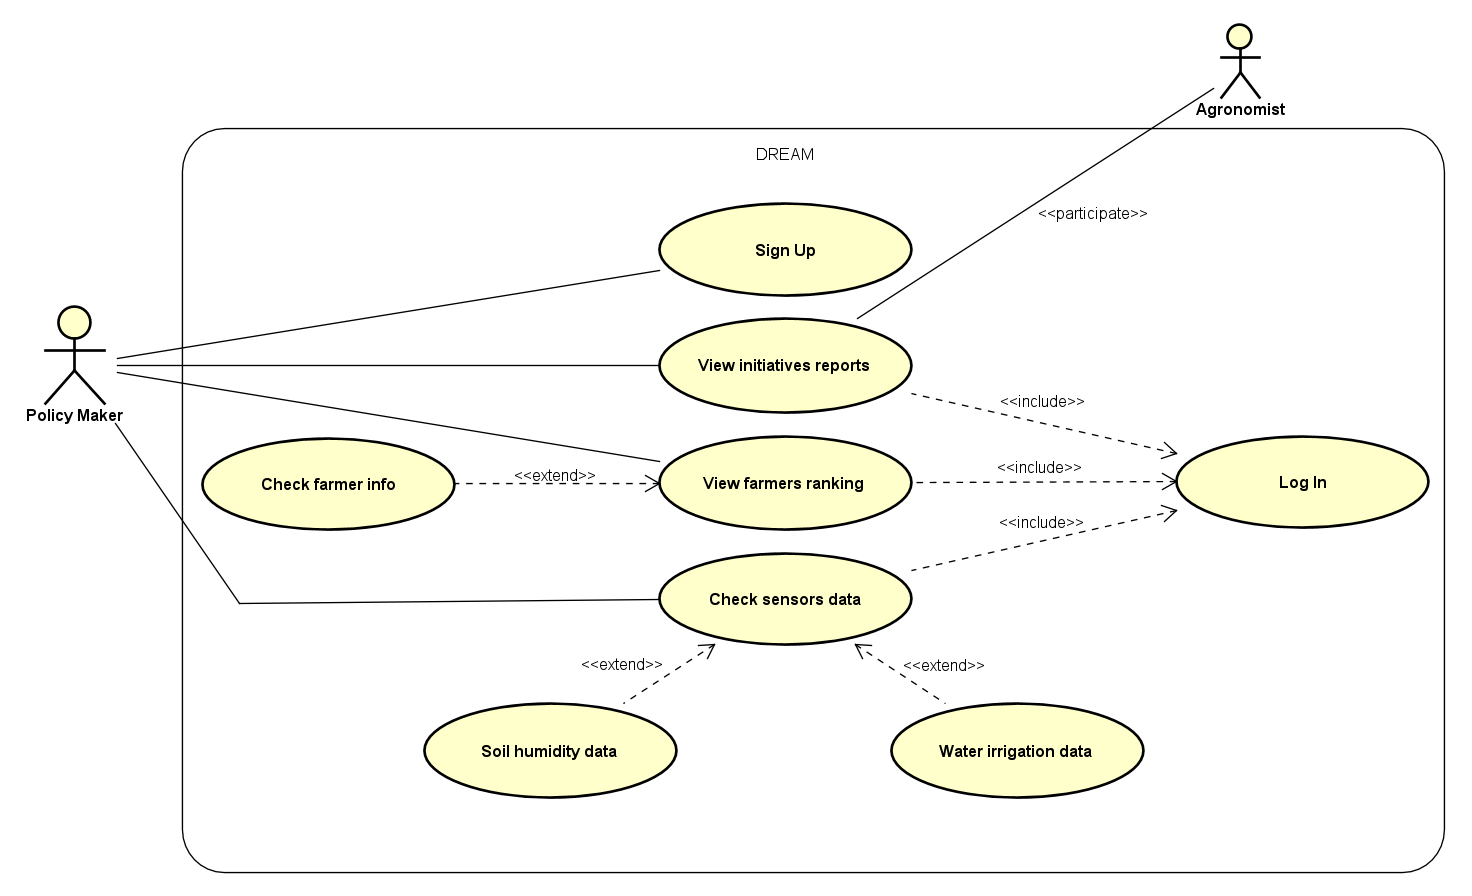
\includegraphics[scale=0.55, center]{assets/Use cases/UseCase_PolicyMaker.png}
            \caption{Policy Maker - Use Case Diagram}
            \label{fig: UseCase_PolicyMaker}
        \end{figure}
    \end{center}
    \newpage
    \item \textbf {Farmers}
    \begin{center}
        \begin{figure}[H]
            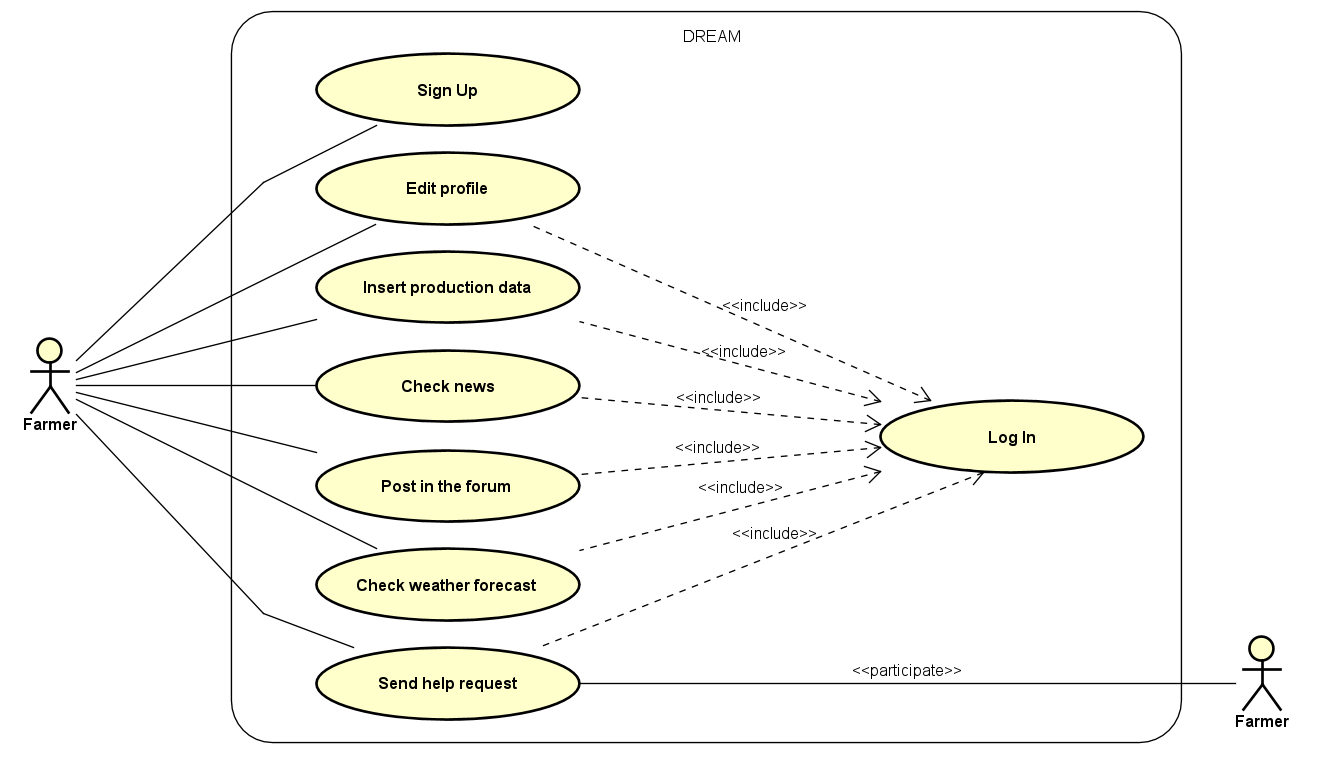
\includegraphics[scale=0.60, center]{assets/Use cases/UseCase_Farmer.png}
            \caption{Farmer - Use Case Diagram}
            \label{fig: UseCase_Farmer}
        \end{figure}
    \end{center}
    \newpage
    \item \textbf {Agronomists}
    \begin{center}
        \begin{figure}[H]
            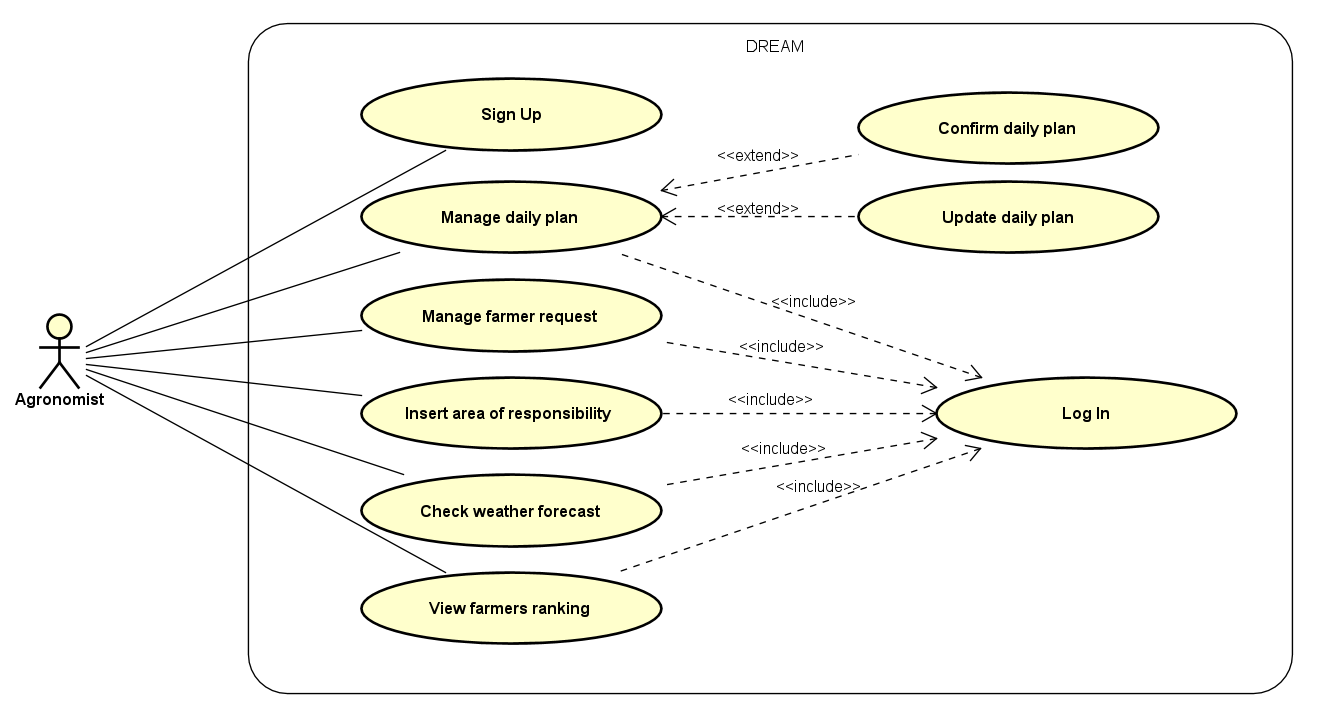
\includegraphics[scale=0.60, center]{assets/Use cases/UseCase_Agronomist.png}
            \caption{Agronomist - Use Case Diagram}
            \label{fig: UseCase_Agronomist}
        \end{figure}
    \end{center}
    \newpage
\end{itemize}

    \paragraph{Use Cases Description}
    
        \begin{itemize}
            \item \textbf {Shared Use Cases}
            
            \begin{table}[H]
                \item[] \textbf{Sign Up}
                \item[] 
                \centering
                \begin{tabular}{|c |m{0.69\textwidth}|}
                    \hline
                    \textbf{Use Case} & Sign Up\\ \hline
                    \textbf{Actor} & Policy Maker, Farmer, Agronomist\\ \hline
                    \textbf{Entry condition} & User wants to register in the system\\  \hline
                    \textbf{Flow of events} & \begin{enumerate}
                                                \item User opens DREAM app
                                                \item User presses the sign up button
                                                \item User selects its username, password and job role
                                                \item User presses the confirm button
                                                \item System shows a confirmation message to the user
                                                \item An email is sent to the user
                                            \end{enumerate}\\ \hline
                    \textbf{Exit condition} & User data are saved into the system and registration ends successfully  \\ \hline
                    \textbf{Exceptions} &  \begin{enumerate}
                        \item If the user insert an already taken username
                        \item If the user press the cancel button
                        \item Internet connection isn't working
                    \end{enumerate}
                    An error message is shown and the flow of events starts again from point 3\\ \hline                    
                \end{tabular}
            \end{table}

            \begin{table}[H]
                \item[] \textbf{Log In}
                \item[]  
                \centering
                \begin{tabular}{|c| m{.69\textwidth}|}
                    \hline
                    \textbf{Use Case} & Log In\\ \hline
                    \textbf{Actor} & Policy Maker, Farmer, Agronomist\\ \hline
                    \textbf{Entry condition} & User wants to log in the system\\  \hline
                    \textbf{Flow of events} & \begin{enumerate}
                                                \item User opens DREAM app
                                                \item User puts its own username and password
                                                \item System correctly log in the user and redirects it the home page
                                            \end{enumerate}\\ \hline
                    \textbf{Exit condition} & The user correctly log in the system\\ \hline
                    \textbf{Exceptions} &  \begin{enumerate}
                        \item If the user inserts a wrong username and password
                        \item Internet connection isn't working
                    \end{enumerate}
                    An error message is shown and the flow of events starts again from point 1\\ \hline                    
                \end{tabular}
            \end{table}

            \newpage
            \item \textbf{Policy Makers}
            
            \begin{table}[H]
                \item[] \textbf{View Initiatives Reports}
                \item[] 
                \centering
                \begin{tabular}{|c| m{.69\textwidth}|}
                    \hline
                    \textbf{Use Case} & View Initiatives Reports\\ \hline
                    \textbf{Actor} & Policy Maker\\ \hline
                    \textbf{Entry condition} & User wants to check the Steering Initiative proposed by agronomists\\  \hline
                    \textbf{Flow of events} & \begin{enumerate}
                                                \item User presses the "View Initiatives Reports" button
                                                \item System retrieves the information
                                                \item System sends to the user the steering initiative insert by the agronomist
                                                \item System displays the data
                                                \item User presses the back button and return to home page
                                            \end{enumerate}\\ \hline
                    \textbf{Exit condition} & User presses the back button \\ \hline
                    \textbf{Exceptions} &   \begin{enumerate}
                        \item Internet connection isn't working
                    \end{enumerate}
                    An error message is shown and the flow of events starts again from point 1\\ \hline                    
                \end{tabular}
            \end{table}
                
            \begin{table}[H]
                \item[] \textbf{Check Soil Humidity Data}
                \item[] 
                \centering
                \begin{tabular}{|c| m{.69\textwidth}|}
                    \hline
                    \textbf{Use Case} & Check Soil Humidity Data\\ \hline
                    \textbf{Actor} & Policy Maker \\ \hline
                    \textbf{Entry condition} & User wants to check the soil humidity data\\  \hline
                    \textbf{Flow of events} & \begin{enumerate}
                                                \item User presses the "Check Sensors Data" button
                                                \item User presess the soil humidity data button
                                                \item System retrieves soil humidity data and send them back to the user
                                                \item System displays the data
                                                \item User presses the home button and return to home page
                                            \end{enumerate}\\ \hline
                    \textbf{Exit condition} & User presses the "Home" button\\ \hline
                    \textbf{Exceptions} &  \begin{enumerate}
                        \item Internet connection isn't working
                    \end{enumerate}
                    An error message is shown and the flow of events starts again from point 1\\ \hline                   
                \end{tabular}
            \end{table}

            \begin{table}[H]
                \item[] \textbf{Check Water Irrigation Data}
                \item[] 
                \centering
                \begin{tabular}{|c| m{.69\textwidth}|}
                    \hline
                    \textbf{Use Case} & Check Water Irrigation Data\\ \hline
                    \textbf{Actor} & Policy Maker \\ \hline
                    \textbf{Entry condition} & User wants to check the water irrigation data\\  \hline
                    \textbf{Flow of events} & \begin{enumerate}
                                                \item User presses the "Check Sensors Data" button
                                                \item User presses the water irrigation button
                                                \item System retrieves water irrigation data and send them back to the user 
                                                \item System displays the data
                                                \item User presses the home button and return to home page
                                            \end{enumerate}\\ \hline
                    \textbf{Exit condition} & User presses the "Home" button\\ \hline
                    \textbf{Exceptions} & \begin{enumerate}
                        \item Internet connection isn't working
                    \end{enumerate}
                    An error message is shown and the flow of events starts again from point 1\\ \hline                   
                \end{tabular}
            \end{table}

            \begin{table}[H]
                \item[] \textbf{View Farmers Ranking}
                \item[] 
                \centering
                \begin{tabular}{|c| m{.69\textwidth}|}
                    \hline
                    \textbf{Use Case} & View Farmers Ranking\\ \hline
                    \textbf{Actor} & Policy Maker\\ \hline
                    \textbf{Entry condition} & User wants to see the farmers ranking\\  \hline
                    \textbf{Flow of events} & \begin{enumerate}
                                                \item User presses the best or the farmers rank widget
                                                \item System retrieves data on farmers ranking
                                                \item System shows ranking data
                                                \item User presses back button and return to home page
                                            \end{enumerate}\\ \hline
                    \textbf{Exit condition} & User press the "Back" button\\ \hline
                    \textbf{Exceptions} &  \begin{enumerate}
                        \item Internet connection isn't working
                    \end{enumerate}
                    An error message is shown and the flow of events starts again from point 1\\ \hline                    
                \end{tabular}
            \end{table}

            \begin{table}[H]
                \item[] \textbf{View Specific Farmer Information (View Farmers Ranking)}
                \item[] 
                \centering
                \begin{tabular}{|c| m{.69\textwidth}|}
                    \hline
                    \textbf{Use Case} & View Specific Farmer information (View Farmers Ranking)\\ \hline
                    \textbf{Actor} & Policy Maker\\ \hline
                    \textbf{Entry condition} & User wants to see the specific information of a farmer\\  \hline
                    \textbf{Flow of events} & \begin{enumerate}
                                                \item First three events are the same of the "View Farmers Ranking" use case 
                                                \item User presses on a farmer name
                                                \item System retrieves farmer data 
                                                \item System displays farmer data
                                                \item User presses back button to return on the rank page
                                            \end{enumerate}\\ \hline
                    \textbf{Exit condition} & User presses "Back" button\\ \hline
                    \textbf{Exceptions} &  \\ \hline                    
                \end{tabular}
            \end{table}
            
            \newpage


            \item \textbf {Farmers}
            
            \begin{table}[H]
                \item[] \textbf{Profile Edit}
                \item[] 
                \centering
                \begin{tabular}{|c |m{.69\textwidth}|}
                    \hline
                    \textbf{Use Case} & Profile Edit\\ \hline
                    \textbf{Actor} & Farmers\\ \hline
                    \textbf{Entry condition} & User wants to modify or update its profile\\  \hline
                    \textbf{Flow of events} & \begin{enumerate}
                                                \item User presses the "Setting" button on its home page
                                                \item User modifies the interest data (username, password, crop type or area)
                                                \item User presses "Confirm" button
                                                \item System applies the change
                                                \item User receives a confirmation message
                                                \item User is redirect to hom epage
                                            \end{enumerate}\\ \hline
                    \textbf{Exit condition} & User receives a confirmation message\\ \hline
                    \textbf{Exceptions} &  \begin{enumerate}
                        \item User choose an already taken username
                        \item User choose the old password
                    \end{enumerate}
                    An error message is shown and the flow of events starts again from point 2\\ \hline                    
                \end{tabular}
            \end{table}

            \begin{table}[H]
                \item[] \textbf{Insert Production Data}
                \item[] 
                \centering
                \begin{tabular}{|c |m{.69\textwidth}|}
                    \hline
                    \textbf{Use Case} & Insert Production Data\\ \hline
                    \textbf{Actor} & Farmers\\ \hline
                    \textbf{Entry condition} & User wants to insert the production data\\  \hline
                    \textbf{Flow of events} & \begin{enumerate}
                                                \item User presses the "Insert Production Data" button
                                                \item User fills the interested fields
                                                \item User press "Confirm" button
                                                \item System collect analiyze and store the data
                                                \item System shows a confirmation message to the user and redirects it to the home page
                                            \end{enumerate}\\ \hline
                    \textbf{Exit condition} & User receives a confirmation message\\ \hline
                    \textbf{Exceptions} &  \begin{enumerate}
                        \item User insert data in a wrong manner
                        \item User press "Back" button
                    \end{enumerate}
                    An error message is shown and the flow of events starts again from point 2\\ \hline                    
                \end{tabular}
            \end{table}
            
            \begin{table}[H]
                \item[] \textbf{Check News}
                \item[] 
                \centering
                \begin{tabular}{|c |m{.69\textwidth}|}
                    \hline
                    \textbf{Use Case} & Check News\\ \hline
                    \textbf{Actor} & Farmers\\ \hline
                    \textbf{Entry condition} & User wants to check the news\\  \hline
                    \textbf{Flow of events} & \begin{enumerate}
                                                \item User press the news box
                                                \item The system retrieve data regarding news 
                                                \item System displays the news
                                                \item User presses the back button
                                            \end{enumerate}\\ \hline
                    \textbf{Exit condition} & User presses "Back" button\\ \hline
                    \textbf{Exceptions} &  \begin{enumerate}
                        \item Internet connection isn't working
                    \end{enumerate}
                    An error message is shown and the flow of events starts again from point 1\\ \hline                    
                \end{tabular}
            \end{table}

            \begin{table}[H]
                \item[] \textbf{Post in the Forum}
                \item[] 
                \centering
                \begin{tabular}{|c| m{.69\textwidth}|}
                    \hline
                    \textbf{Use Case} & Post in the Forum\\ \hline
                    \textbf{Actor} & Farmers\\ \hline
                    \textbf{Entry condition} & User wants to post in the forum\\  \hline
                    \textbf{Flow of events} & \begin{enumerate}
                                                \item User presses "Forum" button
                                                \item User chooses a thread to reply in or the creation of new thread
                                                \item User writes the text
                                                \item User presses the "Post" button
                                                \item System shows a confirmation message and redirects the user to the "Forum" page
                                                \item User presses "Back" button and returns to home page 
                                            \end{enumerate}\\ \hline
                    \textbf{Exit condition} & User presses "Back" button\\ \hline
                    \textbf{Exceptions} &  \begin{enumerate}
                        \item User exceed the maximum number of character 
                        \item Internet connection isn't working
                    \end{enumerate}
                    An error message is shown and the flow of events starts again from point 2\\ \hline                    
                \end{tabular}
            \end{table}

            \begin{table}[H]
                \item[] \textbf{Check Weather Forecast}
                \item[] 
                \centering
                \begin{tabular}{|c |m{.69\textwidth}|}
                    \hline
                    \textbf{Use Case} & Check Weather Forecast\\ \hline
                    \textbf{Actor} & Farmers\\ \hline
                    \textbf{Entry condition} & User wants to check weather forecast\\  \hline
                    \textbf{Flow of events} & \begin{enumerate}
                                                \item User presses on the weather forecast widget
                                                \item System retirves weather data 
                                                \item System displays data
                                                \item User presses the home button and returns to home page
                                            \end{enumerate}\\ \hline
                    \textbf{Exit condition} & User presses "Home" button\\ \hline
                    \textbf{Exceptions} & \begin{enumerate}
                        \item Internet connection isn't working
                    \end{enumerate}
                    An error message is shown and the flow of events starts again from point 1\\ \hline                    
                \end{tabular}
            \end{table}

            \begin{table}[H]
                \item[] \textbf{Send an Help Request}
                \item[] 
                \centering
                \begin{tabular}{|c |m{.69\textwidth}|}
                    \hline
                    \textbf{Use Case} & Send an Help Request\\ \hline
                    \textbf{Actor} & Farmers\\ \hline
                    \textbf{Entry condition} & User needs the agronomist help\\  \hline
                    \textbf{Flow of events} & \begin{enumerate}
                                                \item User presses "Contact Agronomist" button
                                                \item User chooses the object of its help request
                                                \item User writes the message
                                                \item User sends the request by pressing "Send request" button
                                                \item System shows a confirmation message and redirects the user to the home page 
                                            \end{enumerate}\\ \hline
                    \textbf{Exit condition} & The system shows a confirmation message to the user \\ \hline
                    \textbf{Exceptions} &  \begin{enumerate}
                        \item User doesn't fill every mandatory boxes
                        \item Internet connection isn't working 
                    \end{enumerate}
                    An error message is shown and the flow of events starts again from point 1\\ \hline                    
                \end{tabular}
            \end{table}

            \newpage
            \item \textbf{Agronomist}
            
            \begin{table}[H]
                \item[] \textbf{Confirm Daily Plan}
                \item[] 
                \centering
                \begin{tabular}{|c| m{.69\textwidth}|}
                    \hline
                    \textbf{Use Case} & Confirm Daily Plan\\ \hline
                    \textbf{Actor} & Agronomist\\ \hline
                    \textbf{Entry condition} & User wants to confirm its daily plan\\  \hline
                    \textbf{Flow of events} & \begin{enumerate}
                                                \item User presses the daily "Daily Plan" button
                                                \item User chooses the farmers that he want to visit during the day
                                                \item User checks if the farmers has at least two visit
                                                \item User confirms the plan with the "Confirm" button
                                                \item System displays a confirmation button and redirects the user to the home page
                                            \end{enumerate}\\ \hline
                    \textbf{Exit condition} & System displays a confirmation message\\ \hline
                    \textbf{Exceptions} &  \begin{enumerate}
                        \item At the end of the year a farmer has less than two visit
                        \item Internet connection isn't working
                    \end{enumerate}
                    An error message is shown and the flow of events starts again from point 1\\ \hline                    
                \end{tabular}
            \end{table}

            \begin{table}[H]
                \item[] \textbf{Update Daily Plan}
                \item[] 
                \centering
                \begin{tabular}{|c| m{.69\textwidth}|}
                    \hline
                    \textbf{Use Case} & Update Daily Plan\\ \hline
                    \textbf{Actor} & Agronomist\\ \hline
                    \textbf{Entry condition} & User wants to update its daily plan\\  \hline
                    \textbf{Flow of events} & \begin{enumerate}
                                                \item User presses the "Daily Plan" button
                                                \item User presses the "Update Daily Plan" button
                                                \item User writes its deviations
                                                \item User add or remove farmers according the daily plan
                                                \item User confirms the plan with the "Confirm" button
                                                \item System diplays a confirmation message and redirects the user to the home page
                                            \end{enumerate}\\ \hline
                    \textbf{Exit condition} & System displays a confirmation message\\ \hline
                    \textbf{Exceptions} &  \begin{enumerate}
                        \item User doesn't fill every mandatory fields
                        \item Internet connection isn't working
                    \end{enumerate}
                    An error message is shown and the flow of events starts again from point 3\\ \hline                    
                    
                \end{tabular}
            \end{table}

            \begin{table}[H]
                \item[] \textbf{Manage Farmers Request}
                \item[] 
                \centering
                \begin{tabular}{|c| m{.69\textwidth}|}
                    \hline
                    \textbf{Use Case} & Manage Farmers Request\\ \hline
                    \textbf{Actor} & Agronomist\\ \hline
                    \textbf{Entry condition} & User wants to reply to a farmer help request\\  \hline
                    \textbf{Flow of events} & \begin{enumerate}
                                                \item System displays the notification of an incoming message
                                                \item User presses the inbox icon
                                                \item User inserts the object
                                                \item User replys the request
                                                \item User sends the message by pressing the "Send" button
                                                \item System displays a confirmation message and redirects the user to the inbox page
                                            \end{enumerate}\\ \hline
                    \textbf{Exit condition} & System displays the user a confirmation message\\ \hline
                    \textbf{Exceptions} &  \begin{enumerate}
                        \item Object field is empty
                        \item Message field is empty 
                        \item User press the "Cancel" button
                        \item Internet connection isn't working   
                    \end{enumerate}
                    An error message is shown and the flow of events starts again from point 2\\ \hline                    
                \end{tabular}
            \end{table}

            \begin{table}[H]
                \item[] \textbf{Insert responsibility Area}
                \item[] 
                \centering
                \begin{tabular}{|c |m{.69\textwidth}|}
                    \hline
                    \textbf{Use Case} & Insert responsibility Area\\ \hline
                    \textbf{Actor} & Agronomist\\ \hline
                    \textbf{Entry condition} & User wants to update its own coverage area\\  \hline
                    \textbf{Flow of events} & \begin{enumerate}
                                                \item User presses the settings button
                                                \item User selects the new responsibility area
                                                \item User presses the "Confirm" button 
                                                \item System displays a confirmation message and redirects the user to the home page
                                            \end{enumerate}\\ \hline
                    \textbf{Exit condition} & System displays a confirmation message\\ \hline
                    \textbf{Exceptions} &  \begin{enumerate}
                        \item User press the "Cancel" button
                        \item User select an already taken area
                        \item Internet connection isn't working
                    \end{enumerate}
                    An error message is shown and the flow of events starts again from point 1\\ \hline                    
                \end{tabular}
            \end{table}

            \begin{table}[H]
                \item[] \textbf{Check Weather Forecast}
                \item[] 
                \centering
                \begin{tabular}{|c |m{.69\textwidth}|}
                    \hline
                    \textbf{Use Case} & Check Weather Forecast\\ \hline
                    \textbf{Actor} & Agronomist\\ \hline
                    \textbf{Entry condition} & User wants to check the weather forecast in its responasbility area \\  \hline
                    \textbf{Flow of events} & \begin{enumerate}
                                                \item User presses the wheather widget
                                                \item System retrieves and display data 
                                                \item System displays the data
                                                \item User presses the home button to return to the home page
                                            \end{enumerate}\\ \hline
                    \textbf{Exit condition} & User presses "Home" button\\ \hline
                    \textbf{Exceptions} &\begin{enumerate}
                        \item Internet connection isn't working
                    \end{enumerate}
                    An error message is shown and the flow of events starts again from point 1 \\ \hline                    
                \end{tabular}
            \end{table}

            \begin{table}[H]
                \item[] \textbf{View Farmers Area Ranking}
                \item[] 
                \centering
                \begin{tabular}{|c |m{.69\textwidth}|}
                    \hline
                    \textbf{Use Case} & View Farmers Area Ranking\\ \hline
                    \textbf{Actor} & Agronomist\\ \hline
                    \textbf{Entry condition} & User wants to see the ranking of farmers in the area\\  \hline
                    \textbf{Flow of events} & \begin{enumerate}
                                                \item User presses the ranking widget 
                                                \item System retrieves and displays the data
                                                \item User presses the back button and returns to the home page
                                            \end{enumerate}\\ \hline
                    \textbf{Exit condition} & User presses "Home" button\\ \hline
                    \textbf{Exceptions} & \begin{enumerate}
                        \item Internet connection isn't working
                    \end{enumerate}
                    An error message is shown and the flow of events starts again from point 1\\ \hline                    
                \end{tabular}
            \end{table}
            
        
        \newpage

        \item \textbf{Use Cases to requirement mapping}
        
        \item[] \begin{longtable}{|p{0.31\textwidth}|p{0.69\textwidth}|}
                    \hline
                    \cellcolor{SpringGreen!50}\textbf{1)Sign Up}\centering & R3) If the IT device is equipped with GPS technology, then the system must suggest the users the area in which they are during the registration phase. In any case, the final decision will be up to the registering user.
                                                                     
                                                                     R2) The system shall allow users to be identified by a username of their choosing.\\\hline
                    \cellcolor{SpringGreen!50}\textbf{2)Log In}\centering & R18) The system shall allow users to be identified by a username of their choosing. \\\hline
                    \cellcolor{SpringGreen!50}\textbf{3)View Initiative Reports}\centering &  R1) The system must allow only registered and logged-in users to use the app.

                                                                                              R6) The system must allow Policy Makers to retrieve all agronomists' steering initiative rep orts uploaded to the database.\\\hline
                    \cellcolor{SpringGreen!50}\textbf{4)Check Soil Humidity Data}\centering &  R1) The system must allow only registered and logged-in users to use the app.

                                                                                               R5) The system must allow Policy Makers to see up-to-date statistic data, accordingly to the database, about water irrigation systems and soil humidity sensors.\\\hline
                    \cellcolor{SpringGreen!50}\textbf{5)Check Water Irrigation Data}\centering &  R1) The system must allow only registered and logged-in users to use the app.

                                                                                                  R7) The system must allow Policy Makers to see up-to-date statistic data, accordingly to the database, about water irrigation systems and soil humidity sensors.\\\hline
                    
                    \cellcolor{SpringGreen!50}\textbf{6)View Farmers Ranking}\centering &  R1) The system must allow only registered and logged-in users to use the app.

                                                                                           R7) The system must give Policy Makers up-to-date ranking of the best and worst performing farmers.

                                                                                           R8) The system must use a fair and scientific score to rank the Farmers in order to represent the real situation.\\\hline
                    \cellcolor{SpringGreen!50}\textbf{7)View Farmers Ranking}\centering &  R1) The system must allow only registered and logged-in users to use the app.

                                                                                           R7) The system must give Policy Makers up-to-date ranking of the best and worst performing farmers.\\\hline
                    \cellcolor{SpringGreen!50}\textbf{8)Profile Edit}\centering &  R1) The system must allow only registered and logged-in users to use the app.\\\hline
                                
                    \cellcolor{SpringGreen!50}\textbf{9)Insert Production Data}\centering & R1) The system must allow only registered and logged-in users to use the app.

                                                                                  R9) The system must let Farmers insert their production information every day.
                                                                                  
                                                                                  R4) The system must inform the user to try later if they are experimenting connectivity issues .\\\hline
                    \cellcolor{SpringGreen!50}\textbf{10)Check news}\centering &  R1) The system must allow only registered and logged-in users to use the app.
                                                                       
                                                                                 R20) The system must present news concerning crop only if relevant to the Farmer's own crop type.\\\hline
                    \cellcolor{SpringGreen!50}\textbf{11)Post in the Forum}\centering &  R1) The system must allow only registered and logged-in users to use the app.
                    
                                                                               R4) The system must inform the user to try later if they are experimenting connectivity issues .
                                                                               
                                                                               R11) The system must allow every user registered as Farmer to access the forum, to create new discussions and to post replies to already existing ones.\\\hline
                    \cellcolor{SpringGreen!50}\textbf{12)Check Weather Forecast}\centering &  R1) The system must allow only registered and logged-in users to use the app.
                    
                                                                                    R19) The system must show weather forecasts relevant to the area concerning the Farmer or the Agronomist.\\\hline
                    \cellcolor{SpringGreen!50}\textbf{13)Send an Help Request}\centering &  R1) The system must allow only registered and logged-in users to use the app.
                    
                                                                                  R10) The system must provide the contact of the agronomist appointed to the area of the Farmer requesting professional help.
                                                                                  
                                                                                  R4) The system must inform the user to try later if they are experimenting connectivity issues .\\\hline
                    \cellcolor{SpringGreen!50}\textbf{14)Confirm Daily Plan}\centering &  R1) The system must allow only registered and logged-in users to use the app.
                    
                                                                                          R14) The system must suggest to the Agronomists which farms to visit (among the ones in their area of competence) while planning the Daily Plan based up on the last visit day following a FIFO policy. Exceptions to the FIFO policy are the farms under-performing, which shall have higher priority.

                                                                                          R15) The system must suggest to the Agronomists only the farms among the ones in their competence area.

                                                                                          R13) The system must allow the Agronomists to add a new schedule for the day each day.
                                                                                        
                                                                                          R16) The system must allow the Agronomists to update their schedule during the day and to confirm the execution before the end of the day.
                                                                                          
                                                                                          R17) The system must register the already uploaded schedule as definitive if the user doesn't confirm the daily plan for day \textit{x} before 23:59 of the day \textit{x}.\\\hline
                    \cellcolor{SpringGreen!50}\textbf{15)Update Daily Plan}\centering &  R1) The system must allow only registered and logged-in users to use the app.
                    
                                                                                         R13) The system must allow the Agronomists to add a new schedule for the day each day.
                                                                                        
                                                                                         R16) The system must allow the Agronomists to update their schedule during the day and to confirm the execution before the end of the day.

                                                                                         R17) The system must register the already uploaded schedule as definitive if the user doesn't confirm the daily plan for day \textit{x} before 23:59 of the day \textit{x}.\\\hline
                    
                    \cellcolor{SpringGreen!50}\textbf{16)Manage Farmers Request}\centering &  R1) The system must allow only registered and logged-in users to use the app.
                    
                                                                                    R12) The system must notify Agronomists of unresolved requests of help from Farmers.\\\hline
                    \cellcolor{SpringGreen!50}\textbf{17)Insert Responsibility Area}\centering &  R1) The system must allow only registered and logged-in users to use the app.
                    
                                                                                        R2) The system must suggest to the users the area in which they are during the registration phase if the IT device is equipped with GPS technology. In any case, the final decision will be up to the registering user\\\hline
                    \cellcolor{SpringGreen!50}\textbf{18)Check Wheather Forecasat}\centering & R1) The system must allow only registered and logged-in users to use the app.
                    
                                                                                     R19) The system must show weather forecasts relevant to the area concerning the Farmer or the Agronomist.\\\hline
                    \cellcolor{SpringGreen!50}\textbf{19)View Farmers Area Ranking}\centering&  R1) The system must allow only registered and logged-in users to use the app.

                                                                                       R8) The system must use a fair and scientific score to rank the Farmers in order to represent the real situation.
                                                                                       
                                                                                       R18) The system must give Agronomists up-to-date ranking of the best and worst performing farmers in their responsibility area.\\\hline
                    
        \end{longtable}
    
    \end{itemize}

        \newpage
        \subsubsection{Sequence Diagrams}
        \begin{itemize}
            \item \textbf{Shared Sequence Diagrams}\\
            
            \textbf{Sign Up}
            \begin{center}
                \begin{figure}[H]
                    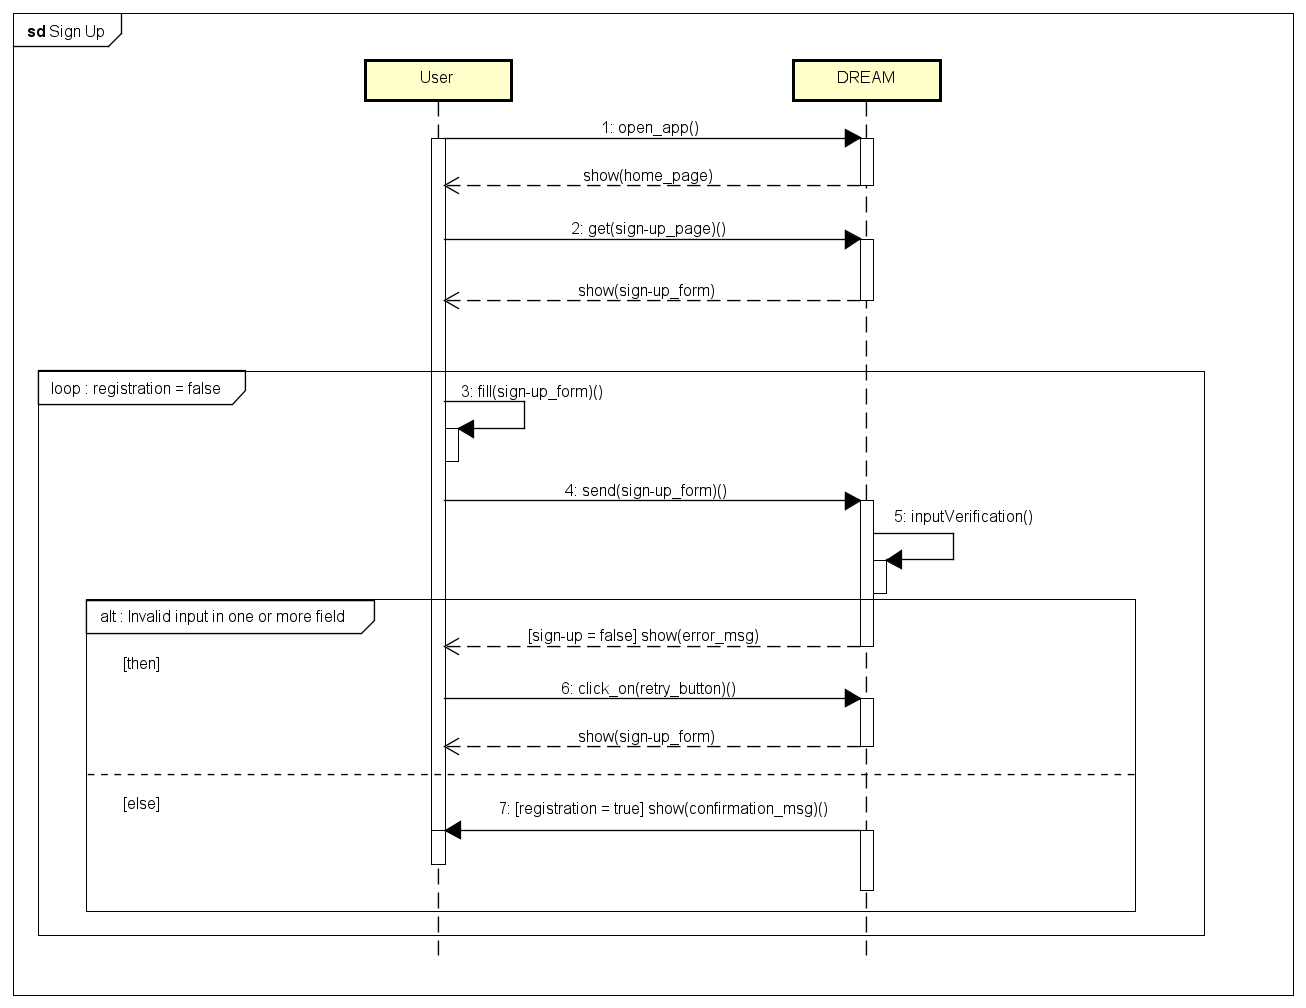
\includegraphics[scale=0.55, center]{assets/Sequence diagrams/Shared/Sign Up.png}
                    \caption{Shared Sequence Diagram - Sign Up Sequence Diagram}
                    \label{fig: sequence_login}
                \end{figure}
            \end{center}

            \textbf{Log In}\\
            \begin{center}
                \begin{figure}[H]
                    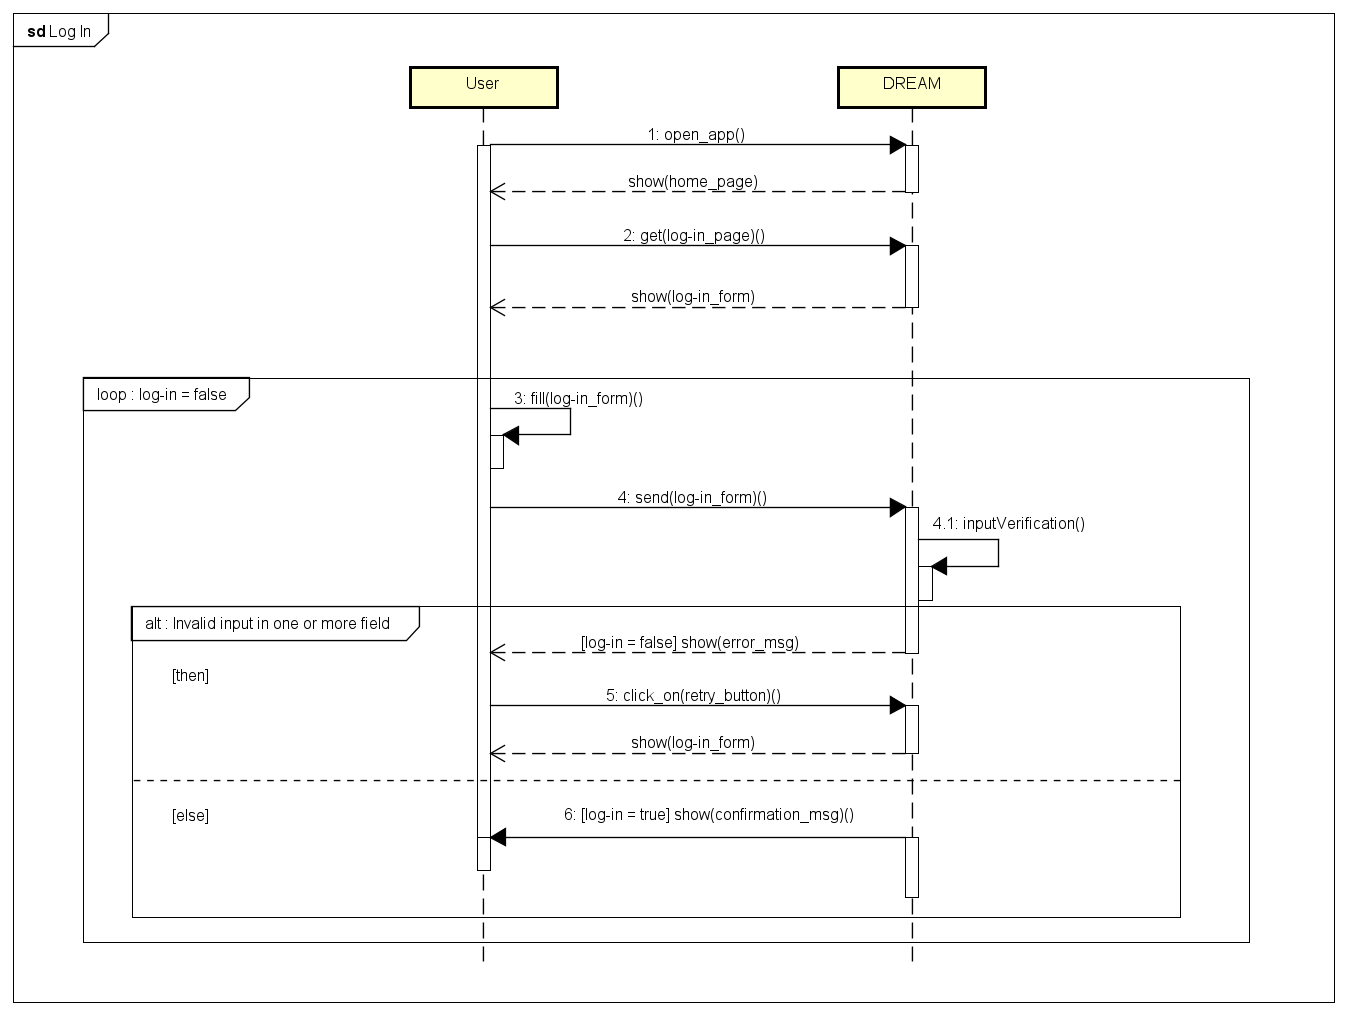
\includegraphics[scale=0.55, center]{assets/Sequence diagrams/Shared/Log In.png}
                    \caption{Shared Sequence Diagram - Log In Sequence Diagram}
                    \label{fig: sequence_login}
                \end{figure}
            \end{center}

            \item \textbf{PolicyMakers}\\
            
            \textbf{View Initiative Report Sequence}\\
            \begin{center}
                \begin{figure}[H]
                    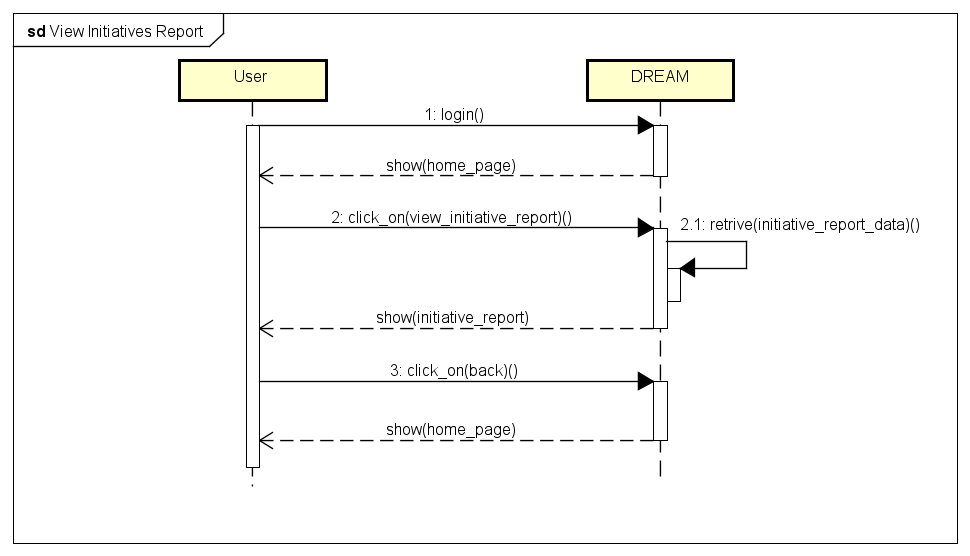
\includegraphics[scale=0.60, center]{assets/Sequence diagrams/Policy Maker/View Initiatives Report.png}
                    \caption{Policy Makers - View Initiative Report Sequence Diagram}
                    \label{fig: sequence_initreport}
                \end{figure}
            \end{center}
            \newpage
            \textbf{Check Soil Humidity Data}\\
            \begin{center}
                \begin{figure}[H]
                    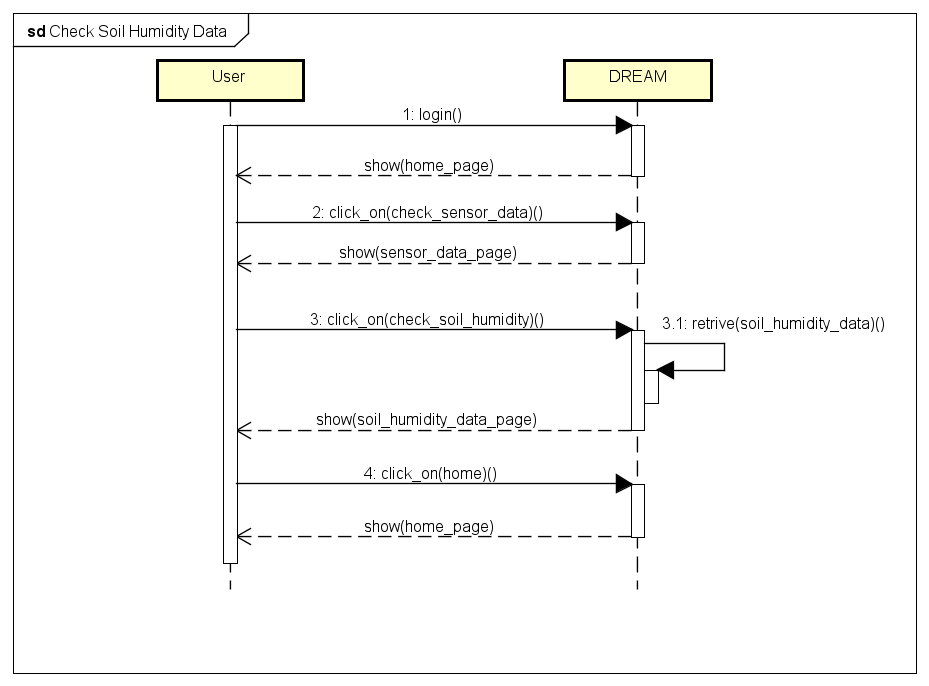
\includegraphics[scale=0.60, center]{assets/Sequence diagrams/Policy Maker/Check Soil Humidity Data.png}
                    \caption{Policy Makers - Check Soil Humidity Data Sequence Diagram}
                    \label{fig: sequence_soil}
                \end{figure}
            \end{center}
            \newpage
            \textbf{Check Water Irrigation Data}\\
            \begin{center}
                \begin{figure}[H]
                    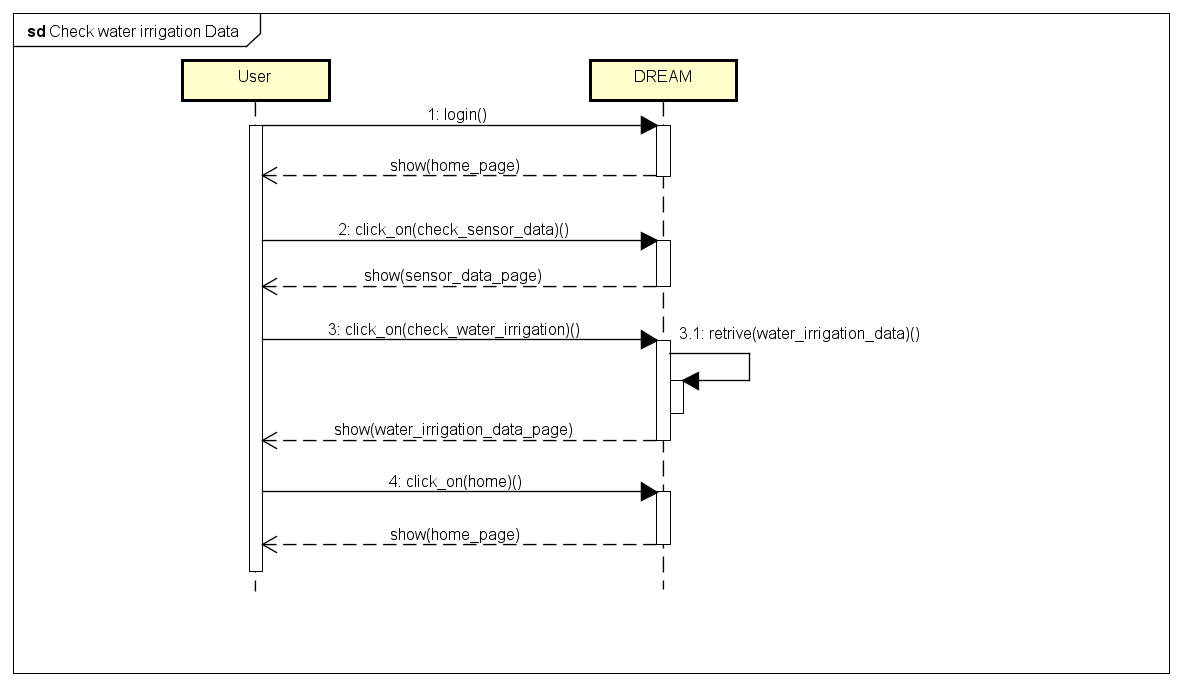
\includegraphics[scale=0.60, center]{assets/Sequence diagrams/Policy Maker/Check Water Irrigation Data.png}
                    \caption{Policy Makers - Check Water Irrigation Data Sequence Diagram}
                    \label{fig: sequence_irrigation}
                \end{figure}
            \end{center}
            \newpage
            \textbf{View Farmers Ranking}\\
            \begin{center}
                \begin{figure}[H]
                    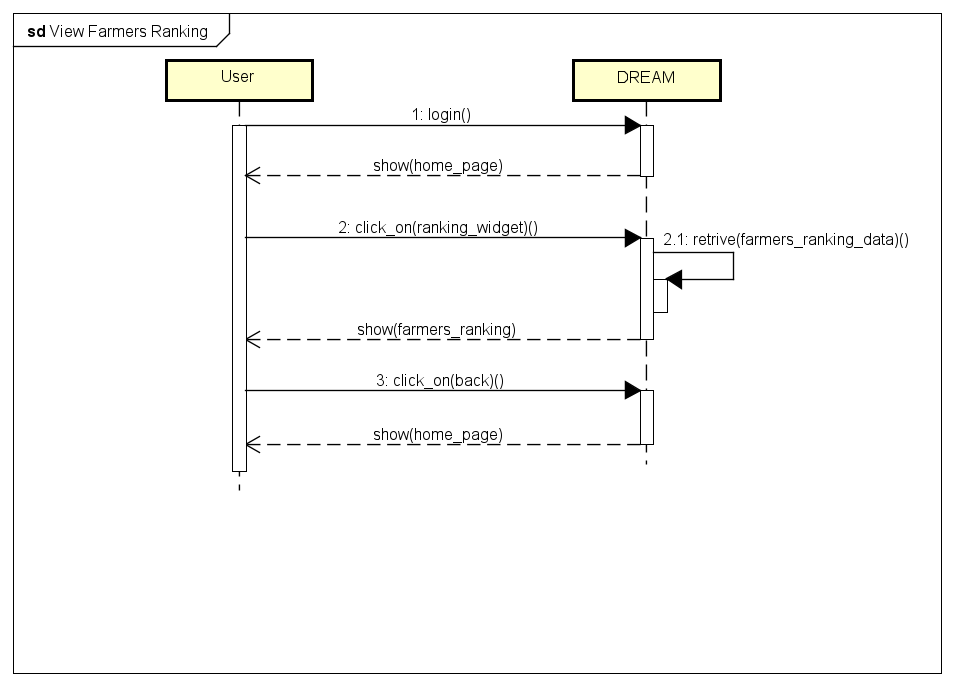
\includegraphics[scale=0.60, center]{assets/Sequence diagrams/Policy Maker/View Farmers Ranking.png}
                    \caption{Policy Makers - View Farmers Ranking Sequence Diagram}
                    \label{fig: sequence_policyrank}
                \end{figure}
            \end{center}
            \newpage
            \textbf{View Specific Farmers information}\\
            \begin{center}
                \begin{figure}[H]
                    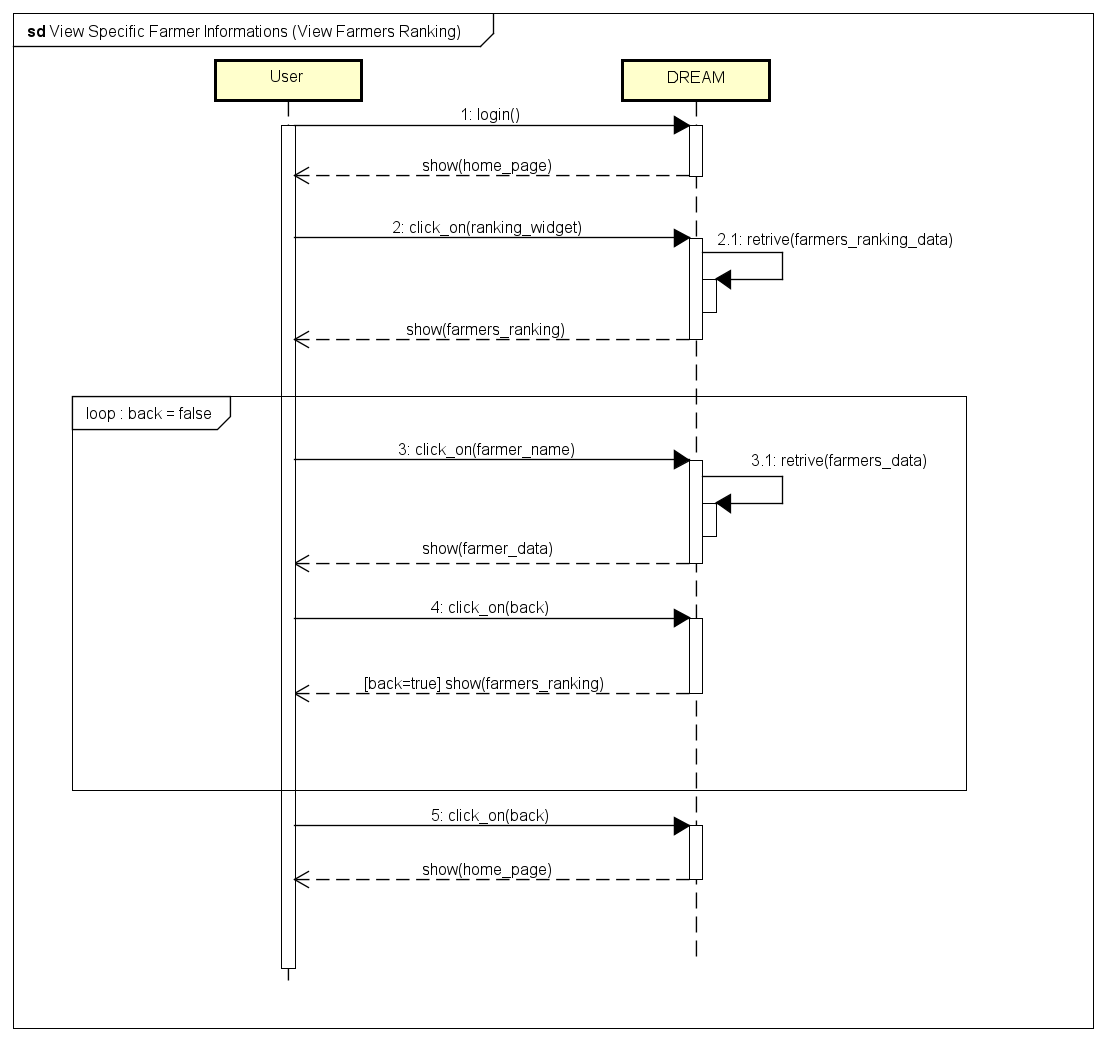
\includegraphics[scale=0.55, center]{assets/Sequence diagrams/Policy Maker/View Specific Farmer Information.png}
                    \caption{Policy Makers - View Specific Farmers information Sequence Diagram}
                    \label{fig: sequence_specificinfo}
                \end{figure}
            \end{center}

            \item \textbf{Farmers}\\
            
            \textbf{Profile Edit}
            \begin{center}
                \begin{figure}[H]
                    %\vspace{-120px}
                    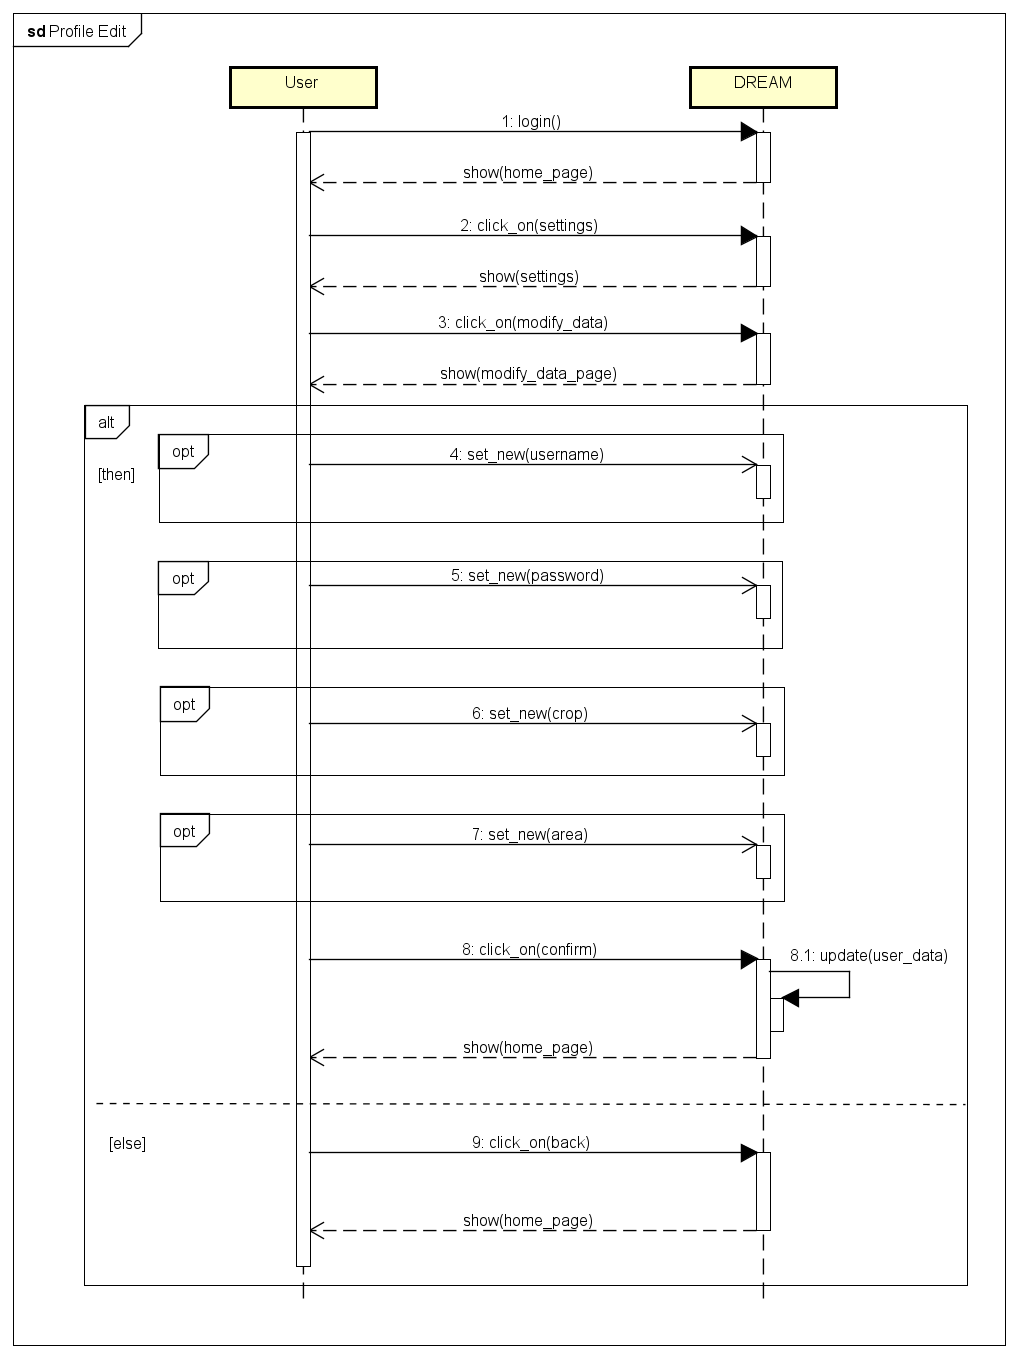
\includegraphics[scale=0.4, center]{assets/Sequence diagrams/Farmer/Profile Edit.png}
                    \caption{Farmers - Profile Edit Sequence Diagram}
                    \label{fig: sequence_editprofile}
                \end{figure}
            \end{center}
            
            
            \textbf{Insert Production Data}
            \begin{center}
                \begin{figure}[H]
                    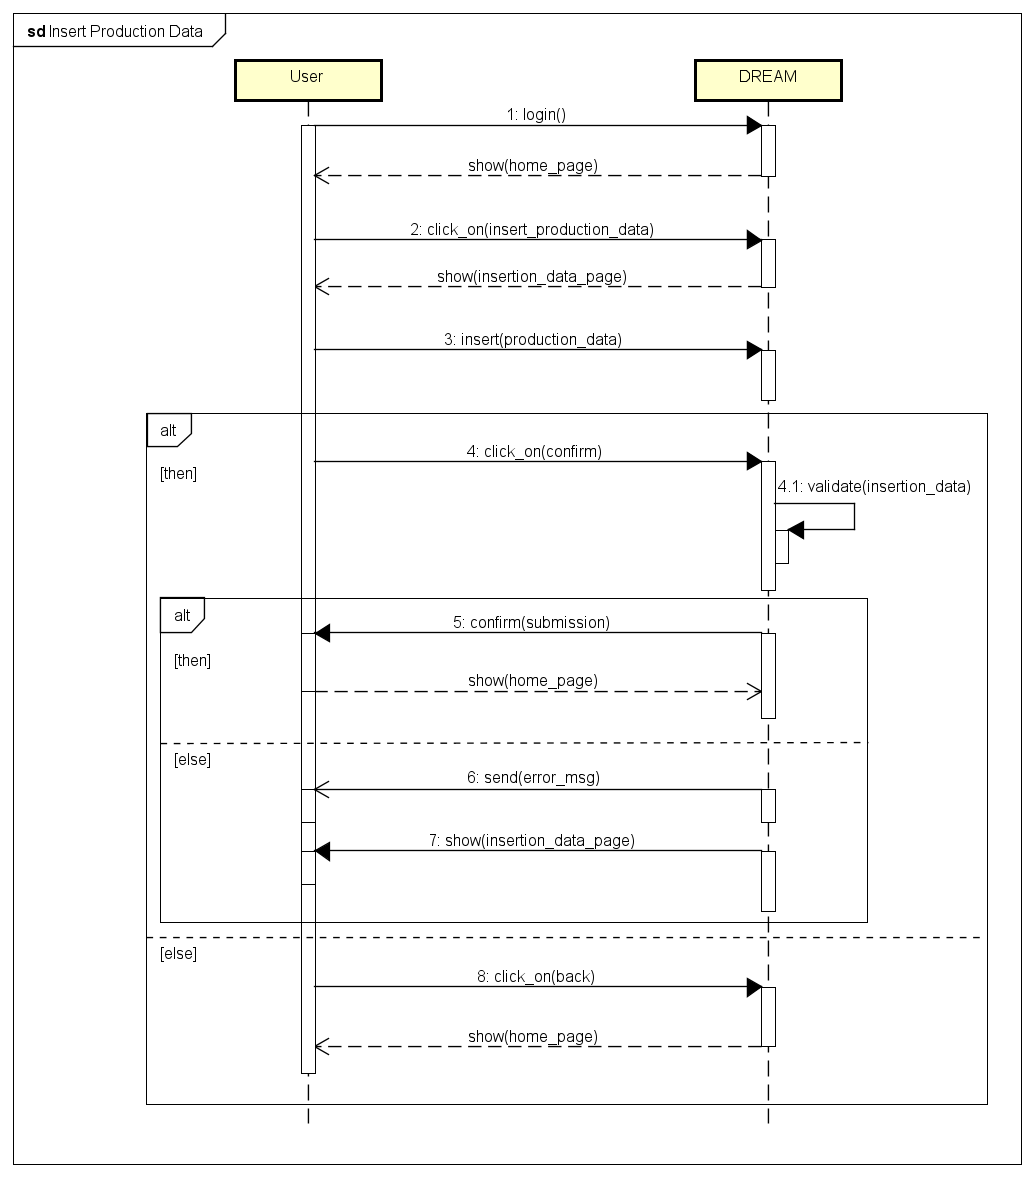
\includegraphics[scale=0.46, center]{assets/Sequence diagrams/Farmer/Insert Production Data.png}
                    \caption{Farmers - Insert Production Data Sequence Diagram}
                    \label{fig: sequence_production}
                \end{figure}
            \end{center}            
            
            \textbf{Check News}\\
            \begin{center}
                \begin{figure}[H]
                    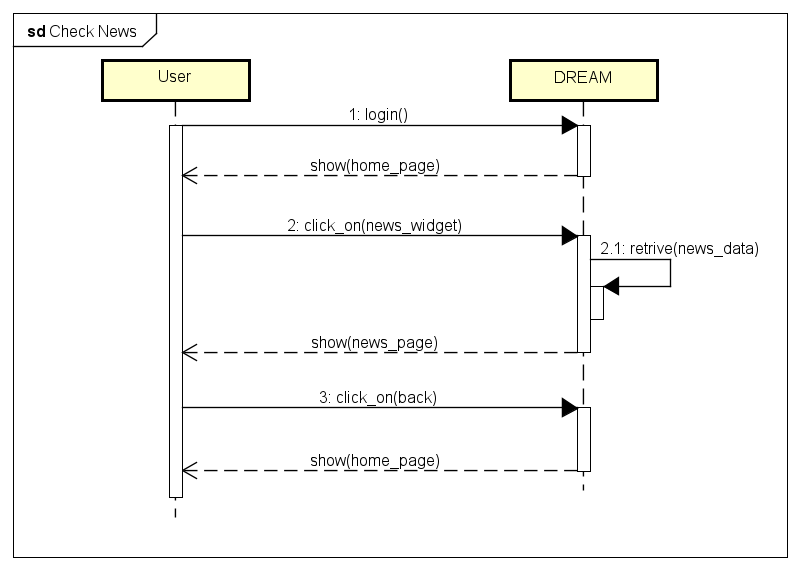
\includegraphics[scale=0.60, center]{assets/Sequence diagrams/Farmer/Check News.png}
                    \caption{Farmers - Check News Sequence Diagram}
                    \label{fig: sequence_news}
                \end{figure}
            \end{center}
            \newpage
            \textbf{Post in the Forum}\\
            \begin{center}
                \begin{figure}[H]
                    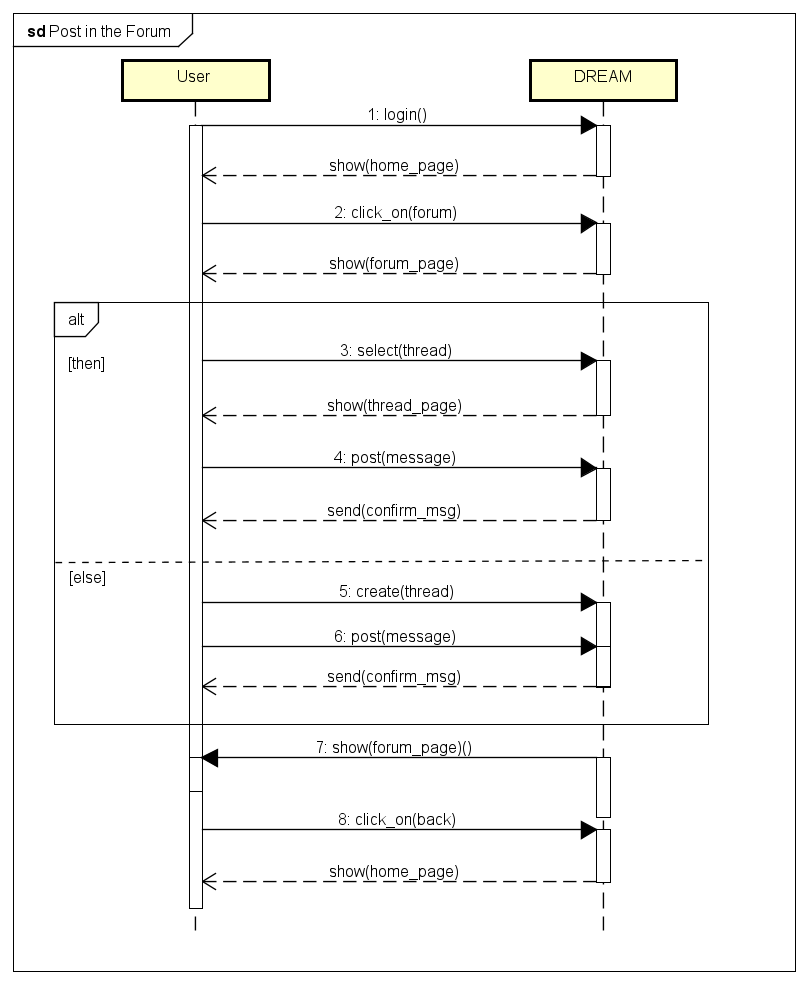
\includegraphics[scale=0.60, center]{assets/Sequence diagrams/Farmer/Post in the Forum.png}
                    \caption{Farmers - Post in the Forum Sequence Diagram}
                    \label{fig: sequence_forum}
                \end{figure}
            \end{center}
            
            \textbf{Check Weather Forecast}\\
            \begin{center}
                \begin{figure}[H]
                    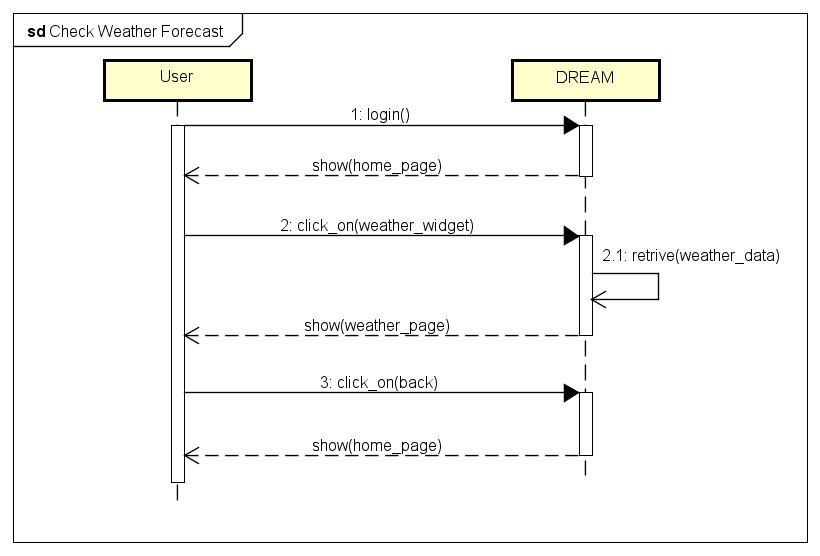
\includegraphics[scale=0.60, center]{assets/Sequence diagrams/Farmer/Check Weather Forecast.png}
                    \caption{Farmers - Check Weather Forecast Sequence Diagram}
                    \label{fig: sequence_weatherfarmers}
                \end{figure}
            \end{center}
            \newpage
            \textbf{Send Help Request}\\
            \begin{center}
                \begin{figure}[H]
                    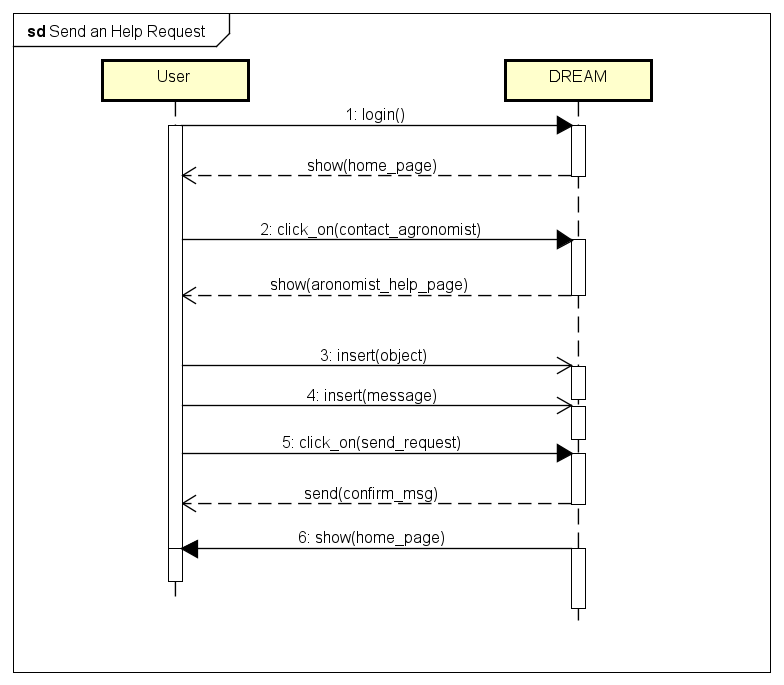
\includegraphics[scale=0.60, center]{assets/Sequence diagrams/Farmer/Send an Help Request.png}
                    \caption{Farmers - Send Help Request Sequence Diagram}
                    \label{fig: sequence_helprequest}
                \end{figure}
            \end{center}

            \newpage
            \item \textbf{Agronomists}\\
            
            \textbf{Confirm Daily Plan}\\
            \begin{center}
                \begin{figure}[H]
                    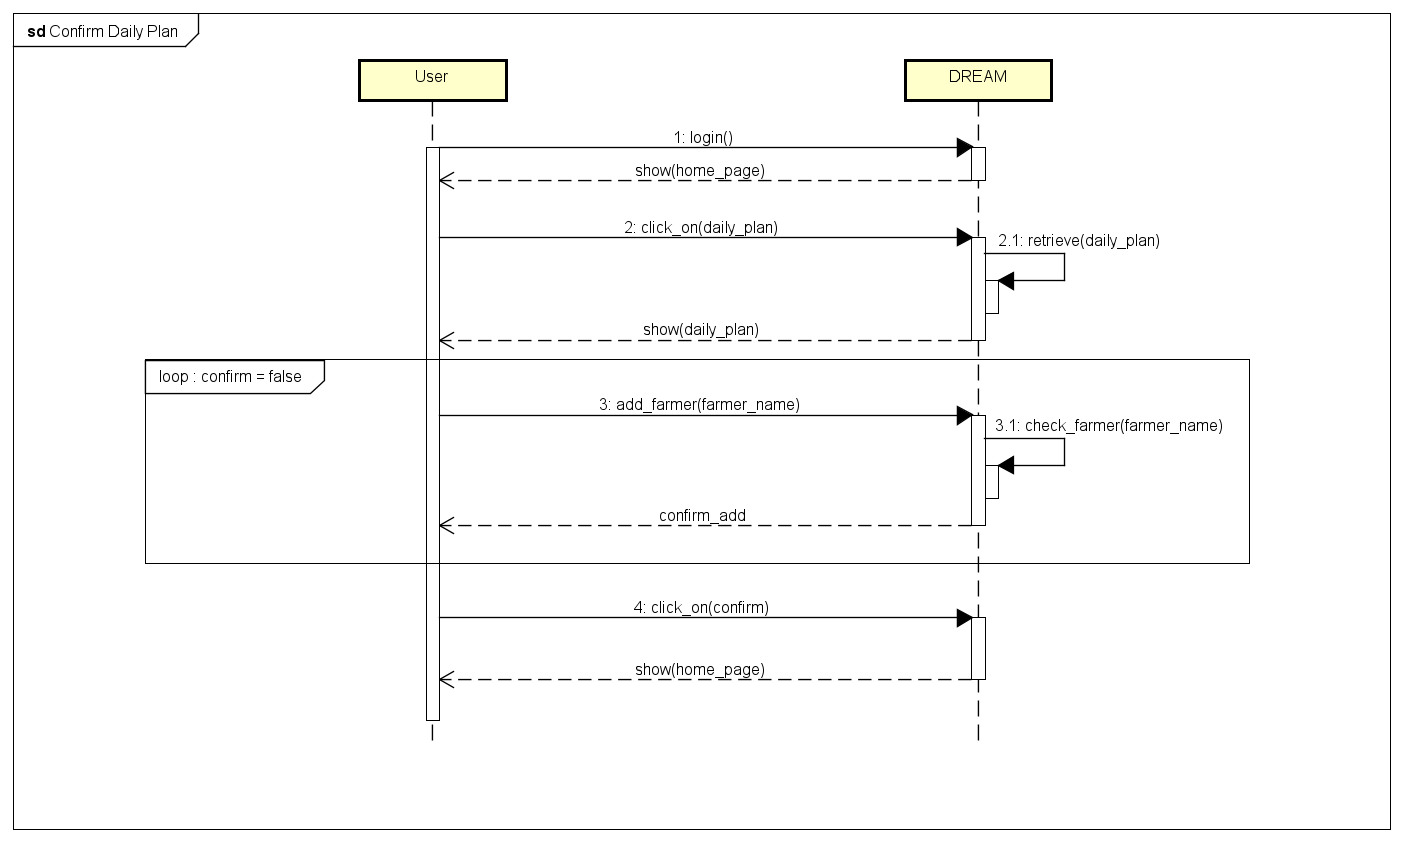
\includegraphics[scale=0.55, center]{assets/Sequence diagrams/Agronomist/Confirm Daily Plan.png}
                    \caption{Agronomists - Confirm Daily Plan Sequence Diagram}
                    \label{fig: sdAgronomist_confirmDailyPlan}
                \end{figure}
            \end{center}
            \newpage
            \textbf{Update Daily Plan}\\
            \begin{center}
                \begin{figure}[H]
                    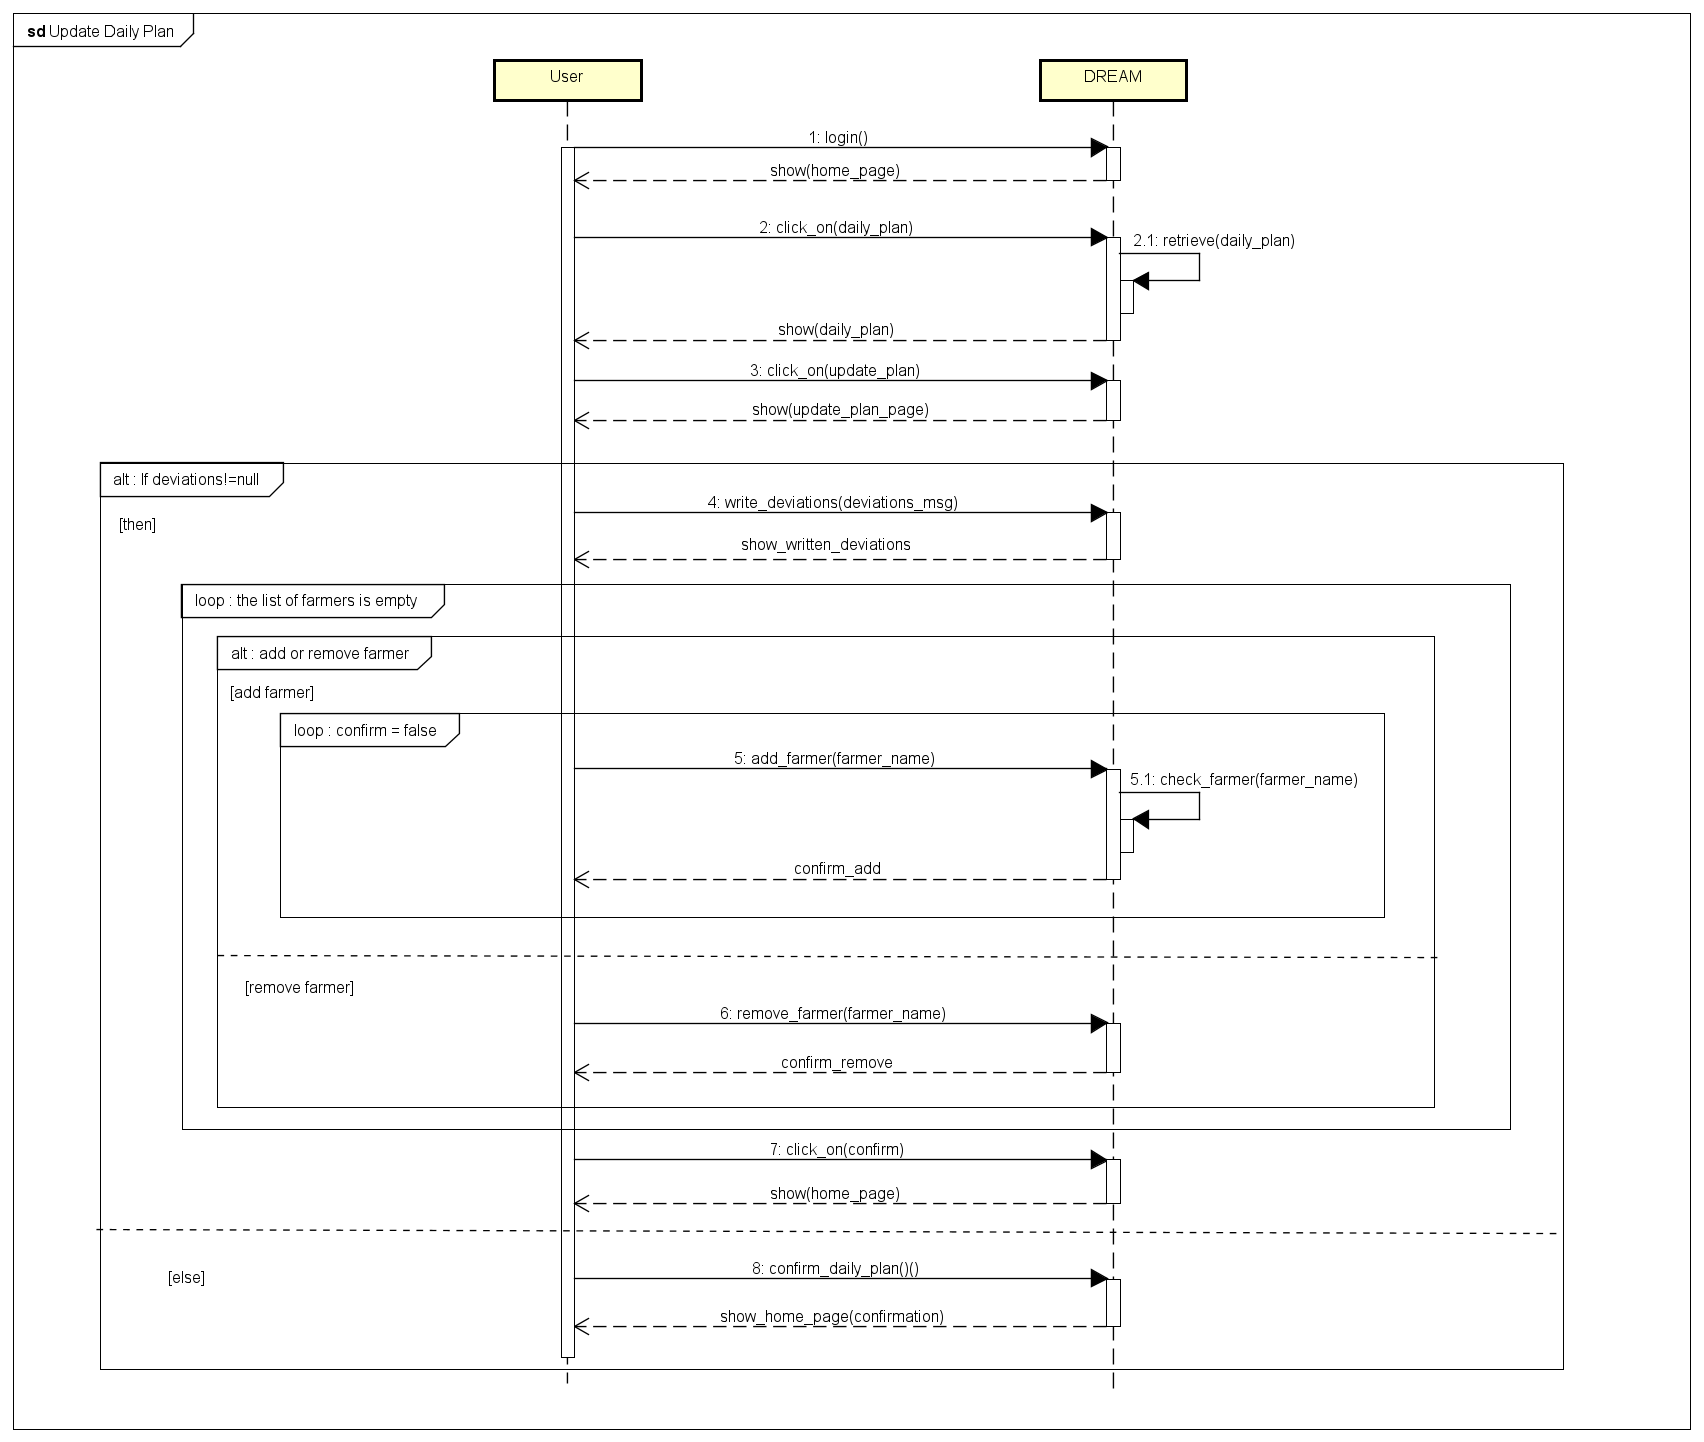
\includegraphics[scale=0.42, center]{assets/Sequence diagrams/Agronomist/Update Daily Plan.png}
                    \caption{Agronomists - Update Daily Plan Sequence Diagram}
                    \label{fig: sdAgronomist_updateDailyPlan}
                \end{figure}
            \end{center}
            \textbf{Manage Farmers Request}\\
            \begin{center}
                \begin{figure}[H]
                    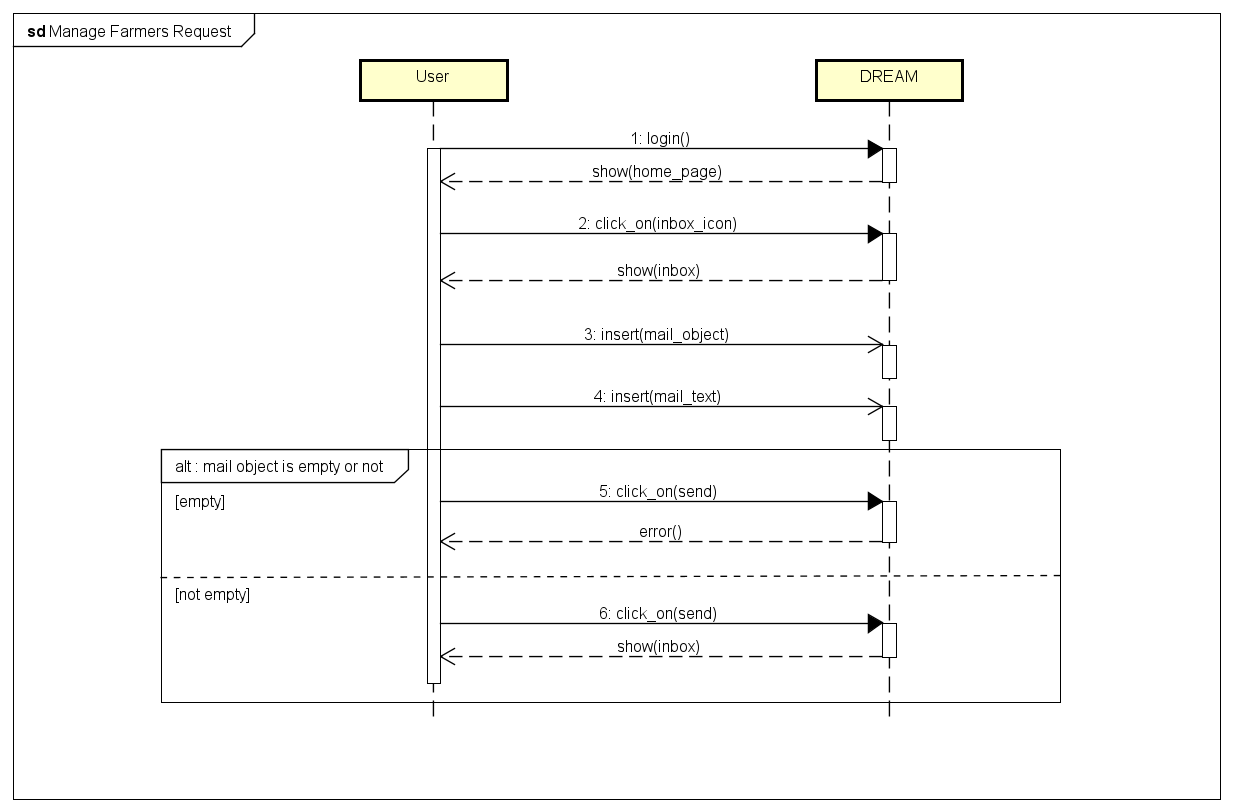
\includegraphics[scale=0.60, center]{assets/Sequence diagrams/Agronomist/Manage Farmers Request.png}
                    \caption{Agronomists - Manage Farmers Request Sequence Diagram}
                    \label{fig: sdAgronomist_manageFarmersRequest}
                \end{figure}
            \end{center}
            \newpage
            \textbf{Insert Responsibility Area}\\
            \begin{center}
                \begin{figure}[H]
                    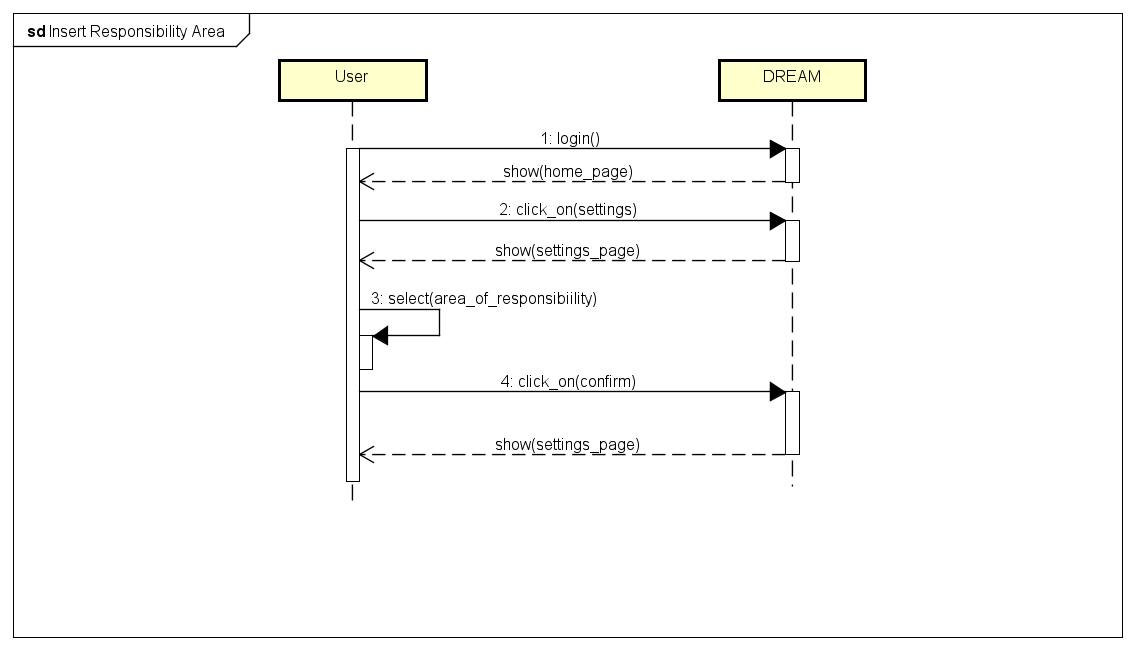
\includegraphics[scale=0.65, center]{assets/Sequence diagrams/Agronomist/Insert Responsibility Area.png}
                    \caption{Agronomists - Insert responsibility Area Sequence Diagram}
                    \label{fig: sdAgronomist_insertResponsibilityArea}
                \end{figure}
            \end{center}
            \newpage
            \textbf{Check Weather Forecast}\\
            \begin{center}
                \begin{figure}[H]
                    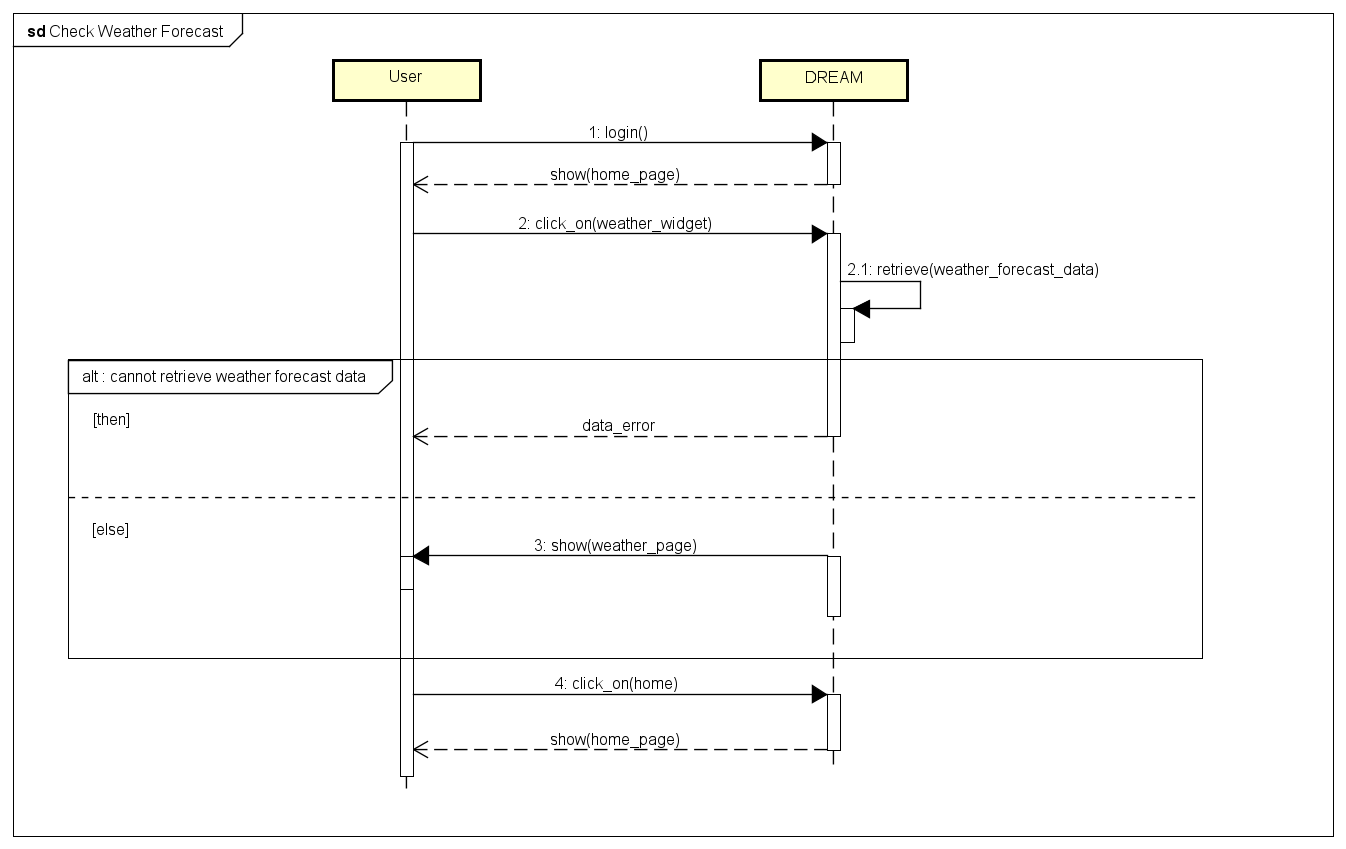
\includegraphics[scale=0.55, center]{assets/Sequence diagrams/Agronomist/Check Weather Forecast.png}
                    \caption{Agronomists - Check Weather Forecast Sequence Diagram}
                    \label{fig: sdAgronomist_checkWeatherForecast}
                \end{figure}
            \end{center}
            \newpage
            \textbf{View Farmers Area Ranking}\\
            \begin{center}
                \begin{figure}[H]
                    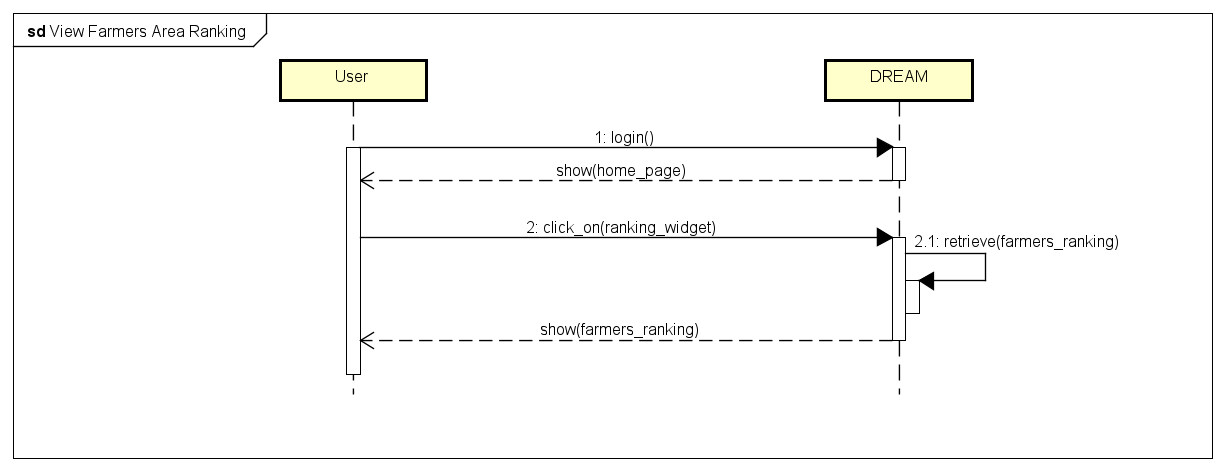
\includegraphics[scale=0.60, center]{assets/Sequence diagrams/Agronomist/View Farmers Area Ranking.png}
                    \caption{Agronomists - View Farmers Area Ranking Sequence Diagram}
                    \label{fig: sdAgronomist_viewFarmersAreaRanking}
                \end{figure}
            \end{center}
        \end{itemize}
        \newpage


\subsection{Performance Requirements}
The majority of the user base will be represented by the farmers that cover the 58\% \cite{specification} of the entire population of Telengana, while the number of policy-maker and agronomist users is irrelevant.
According to Unique Identification Aadhar India, Telangana population in 2021 is estimated to be 39.9 million\cite{population}.
This means that the system is expected to be widely adopted with the registration of millions of users just in the first year.
Also the average workload of the system is expected to be high, the goal is to guarantee the simultaneous connection of at least 2 millions of individuals.
A mid-term goal could be to improve the scalability of the system in order to guarantee an efficient service to all users.
Finally the system should have a good response time, less than 3 seconds is reasonable.
\subsection{Design Constraints}

\subsubsection{Standards compliance}
DREAM's user data must be treated respecting the law according to the PDPA\cite{pdpa}.
\subsubsection{Hardware limitations}
The software is designed to enhance the portability, in fact it is enough to have a device with a stable internet connection.
In order to use the application correctly it is required to have a device equipped with GPS.
%\subsubsection{Any other constraint}

\subsection{Software System Attributes}
\subsubsection{Reliability}
To ensure data consistency the system must have a fully backup infrastructure, this allows to recover from general failures in the main system.
The four components shown in the \textit{Figure(\ref{fig: availability})} operate in parallel, this guarantees high reliability and the correct functioning of the overall system in the case of a single component failure.
Finally all the components of the system must be characterized by the highest MTTF and by the lowest MTTR possible.

\subsubsection{Availability}
The system should be up almost 24/7 in order to allow users to use the application's services at any time.
The peak of use is expected during the working hours, it means that it is better to do all the maintainance activities during the night hours.

\begin{center}
    \begin{figure}[!h]
        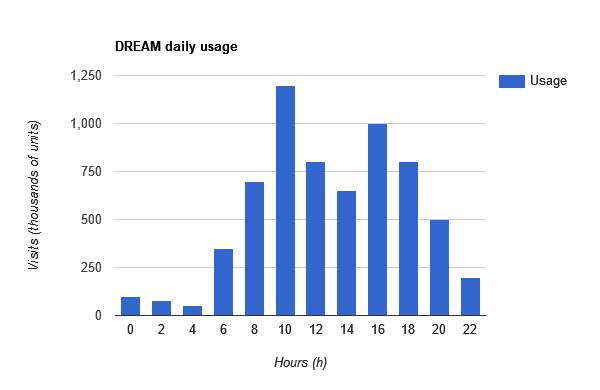
\includegraphics[scale=0.60, center]{assets/bar-graph-daily-usage.png}
        \caption{DREAM daily usage}
        \label{fig: daily_usage}
    \end{figure}
\end{center}

\begin{center}
    \begin{figure}[!h]
        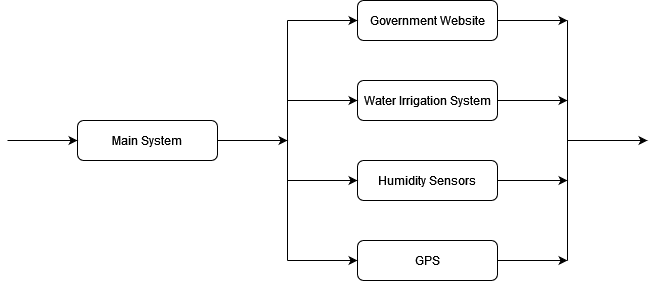
\includegraphics[scale=0.60, center]{assets/Availability.png}
        \caption{DREAM combined availability}
        \label{fig: availability}
    \end{figure}
\end{center}

\begin{table}[H]
    \begin{center}
      \label{tab:availability}
      \begin{tabular}{l|c|r}
        \textbf{Component} & \textbf{Availability} & \textbf{Downtime}\\
        \hline
        Main System & 99.999\% (5-nines) & 5 minutes/year\\
        Government Website & 99.9\% (3-nines) & 8.76 hours/year\\
        Water Irrigation System & 99.9\% (3-nines) & 8.76 hours/year\\
        Humidity Sensors & 99\% (2-nines) & 3.65 days/year\\
        GPS & 99.999\% (5-nines) & 5 minutes/year\\
        \hline
        Entire System & 99.998\% & 10 minutes/year
      \end{tabular}
    \end{center}
\end{table}

\subsubsection{Security}
All the data stored by the system must be encrypted with a standard algorithm like the AES (Advanced Encryption Standard).
The communication passes through a secure channel powered by the SSL protocol.
All data should be stored in compliance with PDPA's regulation.
\subsubsection{Maintainability}
The maintainability is guaranteed by high standard of code, the use of design patterns will enhance this point and guarantee high reusability.
The code must be extensively tested.
The system must be extendible in order to support future updates.
User's application will be regularly updated.
\subsubsection{Portability}
The system is designed to work on different operating systems like Windows, MacOS and Linux.
All main browsers are supported.
\newpage
\section{Formal Analysis using Alloy}
\subsection{Formal Analysis Purpose}
The following analysis aims to formally prove the correctness of the system model by exploiting Alloy verification tool. To achieve so, we test the model by checking if some of the previous defined goals are met. 

Specifically, we stress:
\begin{itemize}
    \item \textbf{(G3) Visualize the result of steering initiatives}: it is modelled as an assertion that checks the ability of the system to retrieve all the reports written by the agronomists and present them to each policy maker.
    \item \textbf{(G4) Visualize relevant data for the farmer business}: the goal is checked by asserting that if and only if there's a news concerning some crop type \textit{x} or a certain area \textit{y}, then the system will present it to all the farmers growing crop type \textit{x} or working in area \textit{y}.
    \item \textbf{(G5) Keep track of the production}: thanks to the predicate, we can formally illustrate the scenario in which a farmer two entries of production are succesfully registered in his/her history production in app (refer to fig. \ref{fig: productionInsertion}).
    \item \textbf{(G6) Request for help/suggestions}: the aim here is to make sure that every farmer that files an help request, there will always be an agronomist (in particular, the one related to the same district where the farm is) that will reply. We show this through an assertion and a predicate that illustarte an instance of this messages' exchange (see fig. \ref{fig: helpRequestAlloy}). Furthermore, we display that some news that are deemed as interesting for a farmer, are actually presented to him/her (refer to fig. \ref{fig: interestingNews}).
    \item \textbf{(G7) Create and participate in discussions concerning the agricolture field}: through two assertions, we make sure that every farmer can create a new topic in the Forum as long as he/she belong to the system and can also join discussions already started by anyone else. Moreover, we make sure thanks to another assertion that each farmer posting something in a dicussion gets automatically linked to the same forum topic. Finally, we show an example of the dynamics that could happen in a forum topic, as shown in fig. \ref{fig: forumDynamics}.
    \item \textbf{(G8) Receive requests of help all in one place}: we check that all the help requests filed by farmers end up in exactly one agronomist's inbox, that is the agronomist whose area of competence matches with the region to which the farmer belongs.
    \item \textbf{(G10) Easy daily planning procedure}: we show an instance of an agronomist's daily plan and we make sure that every farm planned to visit is in the same region of competence of the agronomist.
\end{itemize}

Plus, we runned some empty predicates \texttt{show} to generate some more general instances of the app system.

\subsection{Alloy Code}
\lstinputlisting[language=alloy]{RASD.als}


Here we present some of the instances satifying the predicates that have been generated by the Alloy Analyser.

\begin{center}
    \begin{figure}[H]
        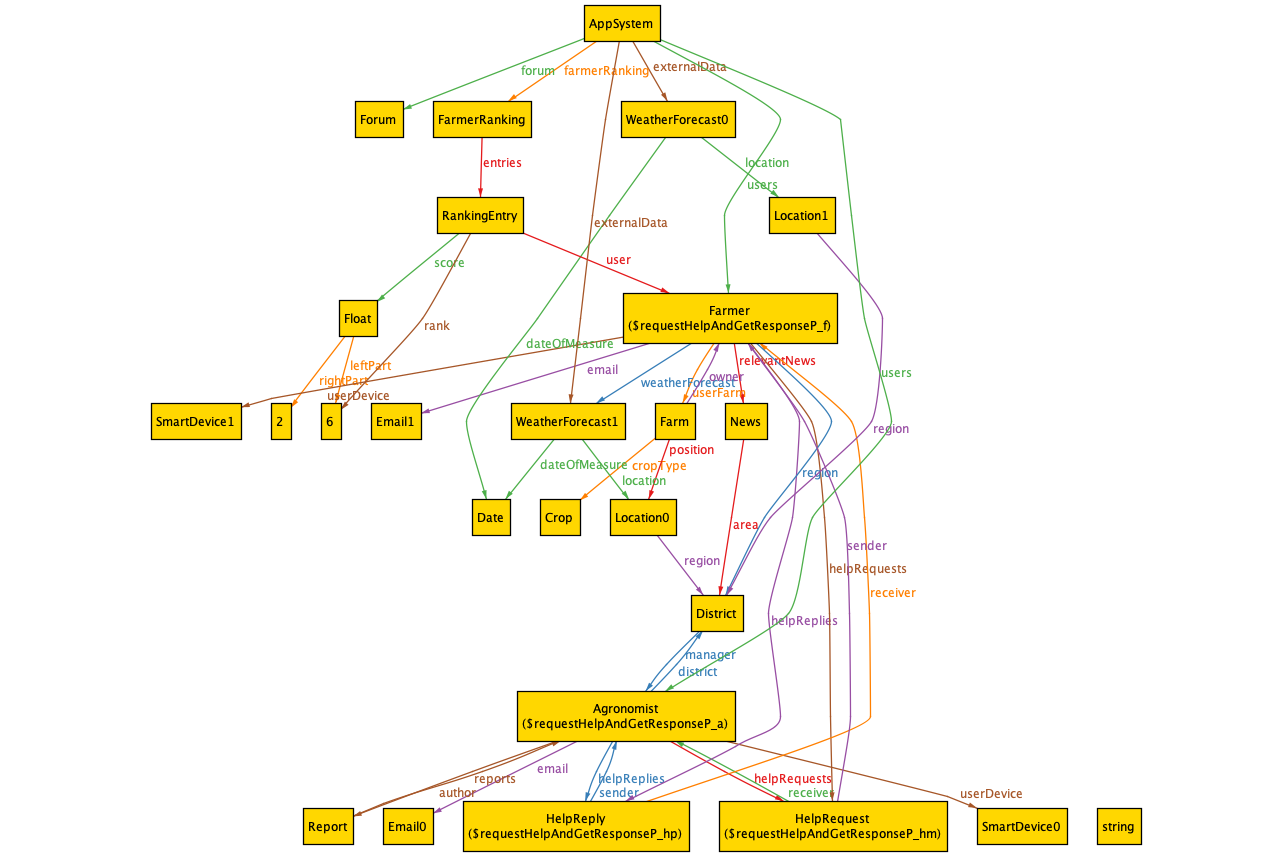
\includegraphics[scale=0.40, center]{assets/AlloyInstances/helpRequests.png}
        \caption{Predicate requestHelpAndGetResponseP}
        \label{fig: helpRequestAlloy}
    \end{figure}
\end{center}

\begin{center}
    \begin{figure}[H]
        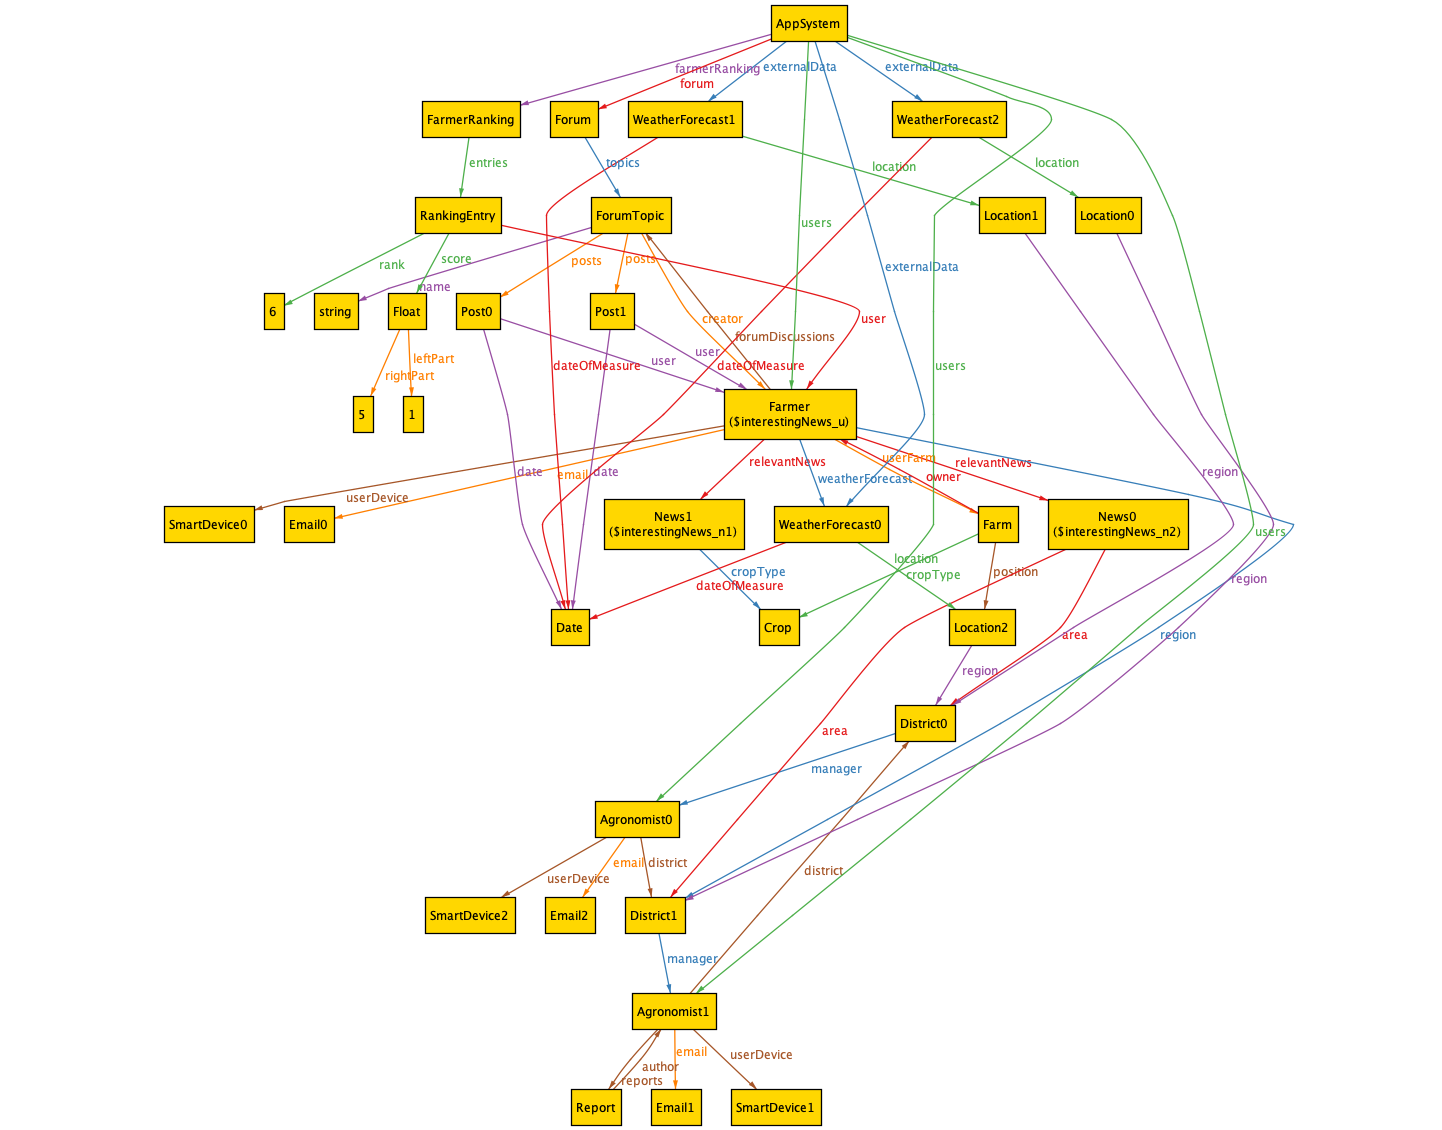
\includegraphics[scale=0.40, center]{assets/AlloyInstances/interestingNews.png}
        \caption{Predicate interestingNews}
        \label{fig: interestingNews}
    \end{figure}
\end{center}

\begin{center}
    \begin{figure}[H]
        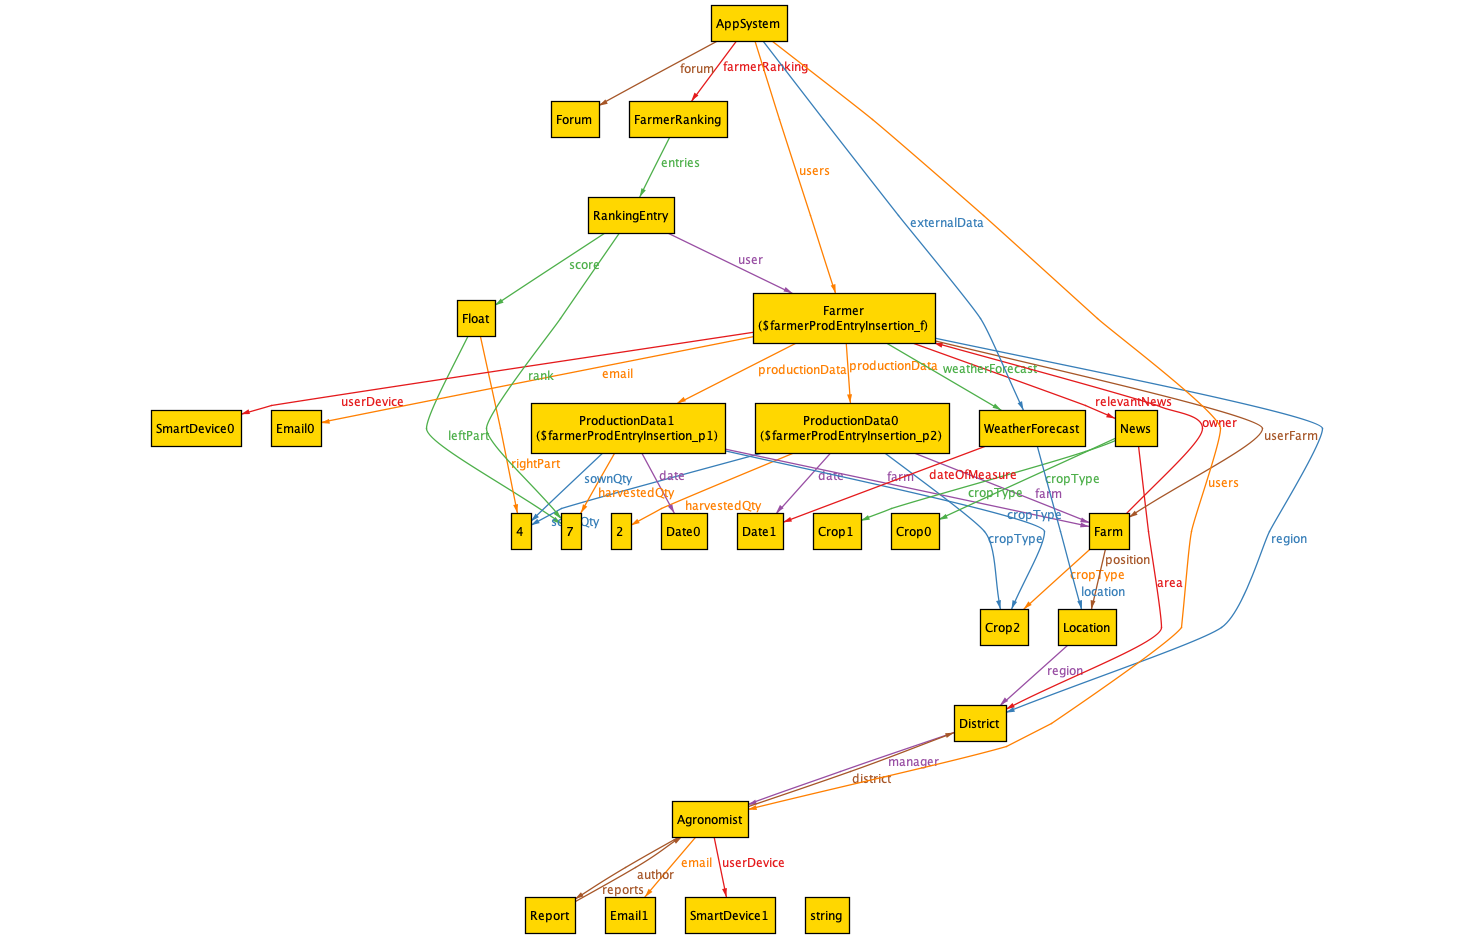
\includegraphics[scale=0.40, center]{assets/AlloyInstances/productionInsertion.png}
        \caption{Predicate farmerProdEntryInsertion}
        \label{fig: productionInsertion}
    \end{figure}
\end{center}

\begin{sidewaysfigure}
    \centering
    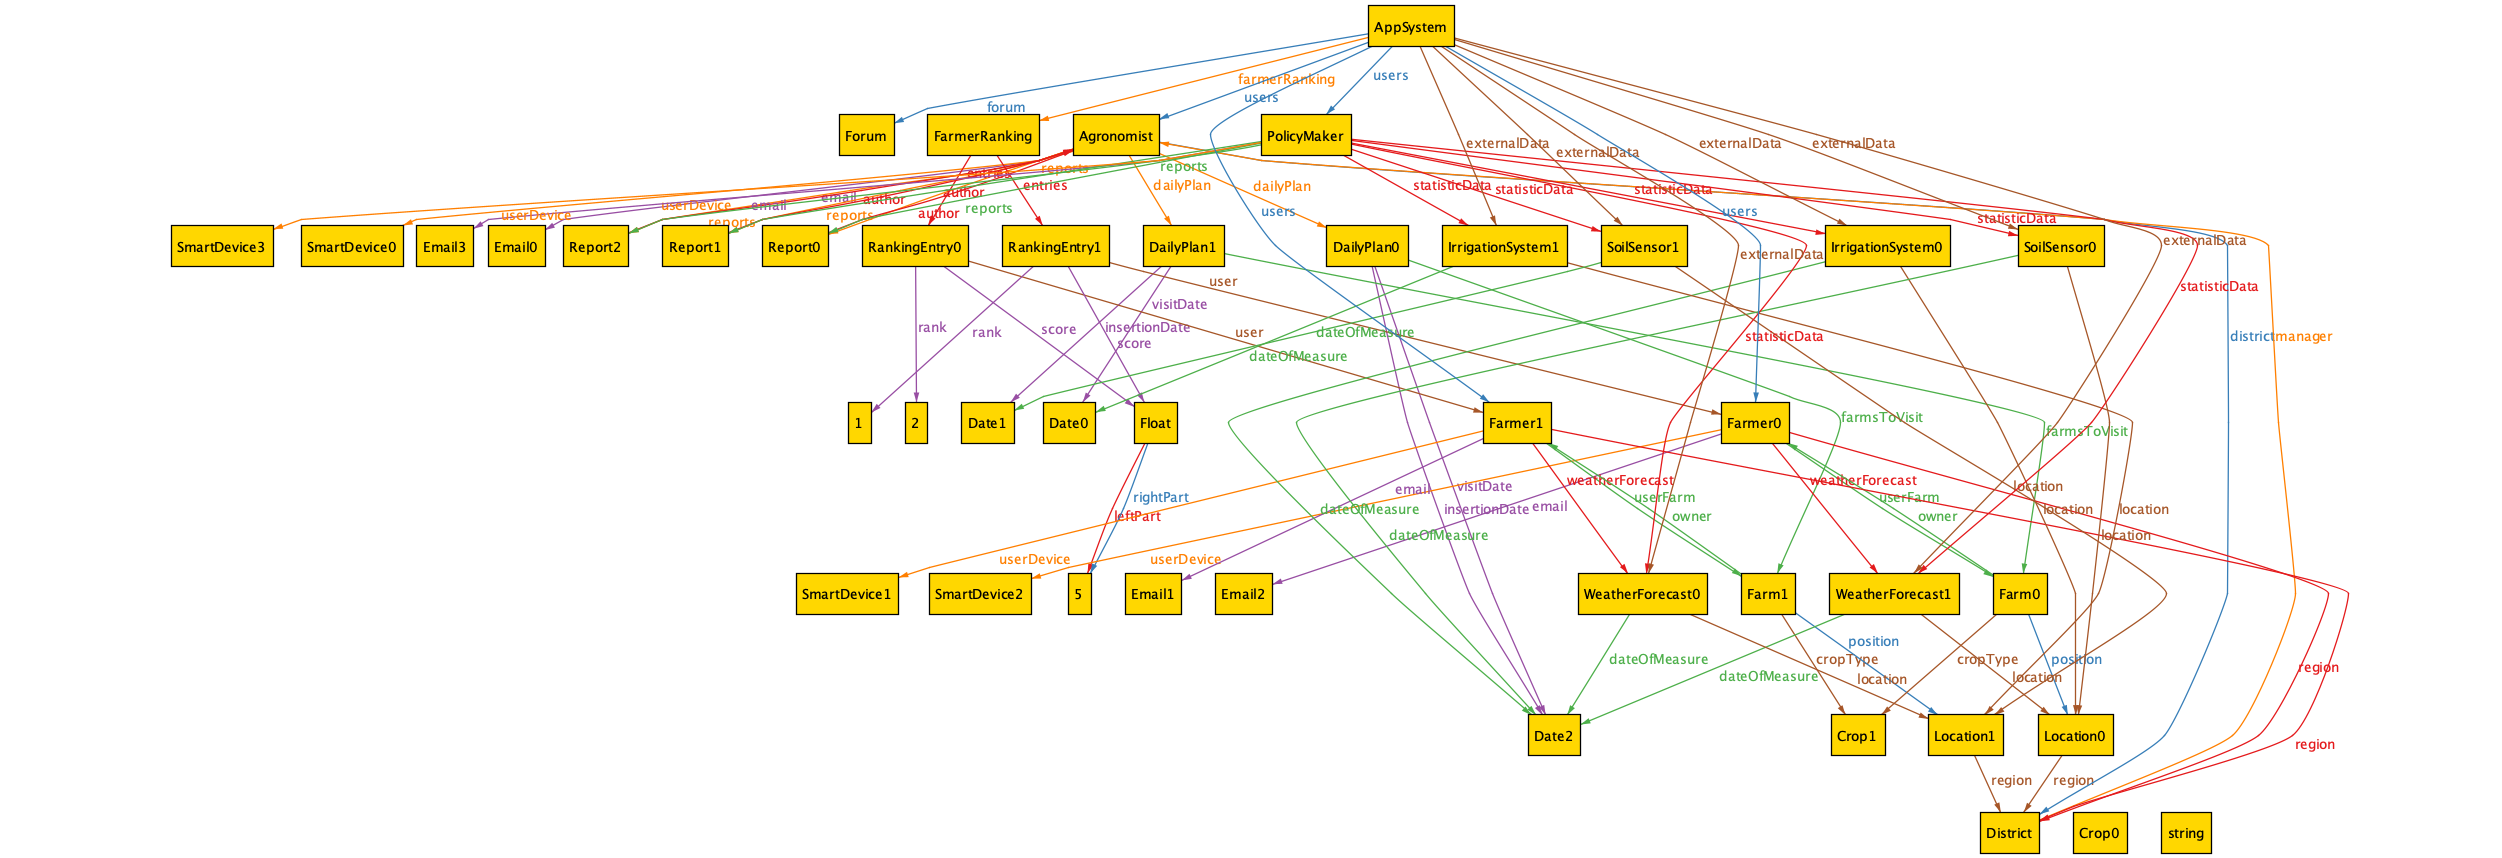
\includegraphics[scale=0.35, center]{assets/AlloyInstances/ExternalData.png}
    \caption{Predicate show focused on external statistic data}
    \label{fig: external data}
\end{sidewaysfigure}

\begin{sidewaysfigure}
    \centering
    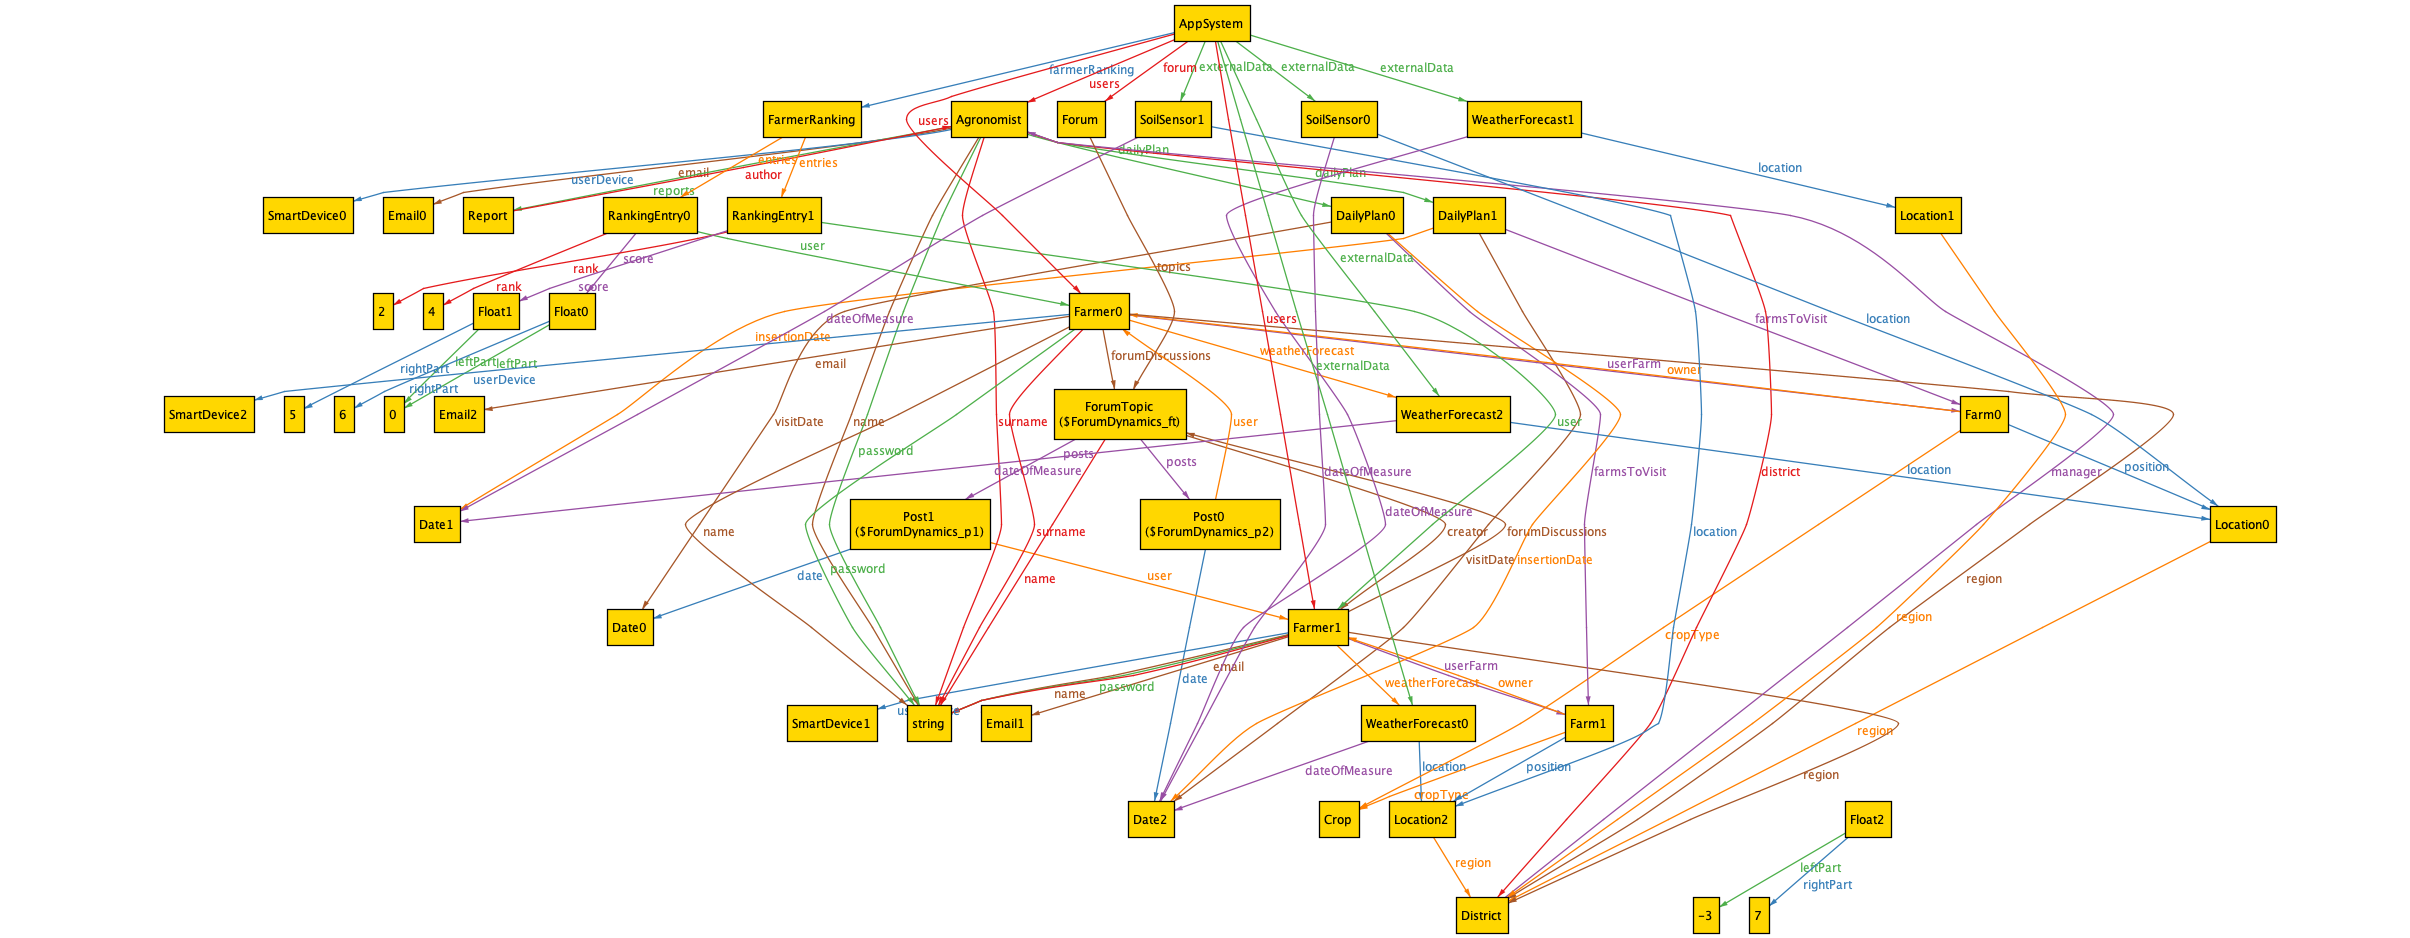
\includegraphics[scale=0.35, center]{assets/AlloyInstances/forumDynamics.png}
    \caption{Predicate forumDynamics}
    \label{fig: forumDynamics}
\end{sidewaysfigure}


\newpage
\section{Effort Spent}
    \begin{tabular}{| c || c | c| c| c |}
        \hline
        Student & Time for S.1 & S.2 & S.3 & S.4 \\ \hline
        Ottavia Belotti & 2.5h & 5h & 11h & 10h \\
        Alessio Braccini & 3h & 6h & 15h & 2h \\
        Riccardo Izzo & 3h & 6h & 15h & 2h \\
        \hline
    \end{tabular}
\section{References}

\begin{thebibliography}{9}
    \bibitem{specification}
    Software Engineering 2,
    \emph{Requirement Engineering and Design Project: goal, schedule and rules}, A.Y. 2021-2022.

    \bibitem{population}
    \url{https://www.populationu.com/in/telangana-population}

    \bibitem{pdpa}
    Indian Ministry of Electronincs and Informations Technology, 
    \url{https://www.meity.gov.in/writereaddata/files/Personal_Data_Protection_Bill,2018.pdf}

\end{thebibliography}

\end{document}